\documentclass[IN,11pt,twoside,openright,master,english]{tumthesis}

% Include common packages
\usepackage{packages}

% IEEE tools for tweaking bib style
\usepackage{IEEEtrantools}

\newcommand\toc{\relax}

\usepackage[backend=bibtex]{biblatex}
\usepackage{booktabs}
\usepackage{tabularx}
\usepackage{longtable}
\usepackage{tabu}
\usepackage{ltxtable}
\usepackage{url}
\usepackage[style=base]{caption}
\captionsetup{%
	font={rm,footnotesize},
	labelfont={sc},
}
\captionsetup[subfloat]{%
	font={rm,footnotesize},
	labelfont={rm},
}
\usepackage{subfig}
\usepackage{nicefrac}
\usepackage{longtable}
\usepackage[hang]{footmisc}
\usepackage{acro}
\usepackage{blindtext}
\usepackage{pgfplots}
\usepackage{colortbl}
\usepackage{booktabs}
\lstset{tabsize=4}

\setlength\footnotemargin{5pt}

% Theorem environments
\newtheorem{definition}{Definition}
\newtheorem{theorem}{Theorem}
\newtheorem{example}{Example}
\newtheorem{lemma}{Lemma}


% hyphenation
\hyphenation{op-ti-cal net-work net-works semi-con-duc-tor tech-nique tech-niques}


\usepackage{mdframed}
\newlength{\charwidth}
\setlength{\charwidth}{\widthof{\scriptsize\texttt{x}}}

\makeatletter
\newenvironment{moeplstborder}[2][]{%
\ifx#1\@empty\@empty%
	\edef\@margin{-1.5\baselineskip}%
\else%
	\edef\@margin{#1}%
\fi%
\vspace{-\baselineskip}
\begin{center}
\begin{minipage}{#2}
\begin{mdframed}[%
	topline=false,leftline=false,bottomline=false,rightline=true,
	linecolor=TUMRed!20,linewidth=\charwidth,
	innertopmargin=\@margin,innerbottommargin=-0.5\baselineskip,
	innerleftmargin=0pt,innerrightmargin=-\charwidth,
	userdefinedwidth=#2,
]%
}%
{%
\end{mdframed}%
\end{minipage}
\end{center}
}%
\makeatother

% Needed for Bachelor's theses, Master's theses and IDP
\titleenglish{MoonWire: Accelerated Site-to-Site VPN}
\titlegerman{MoonWire: Beschleunigtes Site-to-Site VPN}
\author{Maximilian~Pudelko}
\supervisor{\NEThead}
\advisor{Prof.~Dr.-Ing.~Wolfgang~Utschick}
\assistants{Paul~Emmeric\tlc{}~M.\,Sc.,%
Sebastion~Gallenmüller\tlc{}~M.\,Sc.}
\courseofstudy{Informatics}
\date{November 15, 2018}
\location{Garching}

\setcounter{tocdepth}{2}

\DeclareAcroListStyle{longtabu}{table}{%
	table = longtabu,
	table-spec = @{}>{}lX@{}
}{%

\acsetup{%
	list-style=longtabu,
	extra-style=plain,	% remove dot after long in list
	only-used=false,
}

\tabulinesep=1ex

\DeclareAcronym{iso}{
	short				= {\sc{ISO}},
	long				= {International Organization for Standardization},
	list				= {\acl{iso}.},
}
\DeclareAcronym{osi}{
	short				= {\sc{OSI}},
	long				= {Open Systems Interconnection},
	list				= {\acl{osi}.},
	extra				= {%
		Reference model for layered network architectures by the \ac{osi}.
	},
}
\DeclareAcronym{pdu}{
	short				= {\sc{PDU}},
	short-plural-form	= {\sc*{PDU}s},
	long				= {protocol data unit},
	long-plural-form	= {protocol data units},
	list				= {\Acl{pdu}.},
	extra				= {%
	Refers to a message at a specific layer of the \acs{osi} model including
	all headers and trailers of the respective layer and all layers above.
	},
}
\DeclareAcronym{sdu}{
	short				= {\sc{SDU}},
	short-plural-form	= {\sc*{SDU}s},
	long				= {service data unit},
	long-plural-form	= {service data units},
	list				= {\Acl{sdu}.},
	extra				= {%
		Refers to the payload of a message at a specific layer of the \acs{osi}
		model excluding all headers and trailers of the respective layer.
	},
}
\DeclareAcronym{mac}{
	short				= {\sc{MAC}},
	long				= {medium access control},
	list				= {\Acl{mac}.},
}
\DeclareAcronym{tcp}{
	short				= {\sc{TCP}},
	long				= {transmission control protocol},
	list				= {\Acl{tcp}.},
	extra				= {%
		Stream-oriented, reliable, transport layer protocol.
	}
}
\DeclareAcronym{udp}{
	short				= {\sc{UDP}},
	long				= {user datagram protocol},
	list				= {\Acl{udp}.},
	extra				= {%
		Datagram-oriented, unreliable transport layer protocol.
	}
}
\DeclareAcronym{sctp}{
	short				= {\sc{SCTP}},
	long				= {Stream Control Transmission Protocol},
	list				= {\acs{sctp}.},
	extra				= {%
		Datagram-oriented, semi-reliable transport layer protocol.
	}
}
\DeclareAcronym{vpn}{
	short				= {\sc{VPN}},
	long				= {Virtual Private Network},
	list				= {\acs{vpn}.},
	extra				= {%
		Extended, secured private network of a public network.
	}
}


%\addbibresource{bib/IEEEfull.bib}
%\addbibresource{bib/litnew.bib}
\addbibresource{bib/mybib.bib}


%\renewcommand{\andothersdelim}{}
%bib.sty does not work older bibtex versions (works on TexLive 2016 or newer)
%\usepackage{bib}

% Load late to avoid same identifier warning
\usepackage[colorlinks=false,pdfborder={0 0 0}]{hyperref}


\begin{document}%

% Makes sure that same author names are not replaced by dahes
\bstctlcite{IEEEexample:BSTcontrol}

\pagenumbering{gobble}
\maketitle%
\cleardoublepage


\begin{abstract}
	\small

\blindtext

\blindtext

\end{abstract}

%\begin{otherlanguage}{ngerman}
%	\begin{abstract}
%		\small

\blindtext

\blindtext

%	\end{abstract}
%\end{otherlanguage}

%\begin{thanks}
%%\input{/home/moepi/.thanks}
%\end{thanks}

%\begin{preface}
%foo bar
%\end{preface}

\tableofcontents


\startcontent
\chapter{Introduction \& Motivation}
\label{chap:intro}

\Acp{vpn} play an important role in todays network infrastructure. %TODO reference
They are used in a multitude of scenarios and by very different actors. Multi-national firms use them to inter-connect their spread locations across the world. 
So the usage ranges from many hundreds (or thousand) of concurrent sessions to just one in the private user setup.

- mobile telephone base station to backbones 
Goal: connect and transmit data over the public Internet

With these many different usage scenarios, a variety of protocols and implementations were developed over the years, each with slightly different opinions about many aspects.

As the amounts of traffic increases over time \cite{DECIX} the implementations handling it must become more efficient at it.
%TODO: Comparison CPU speed vs. traffic increase (vs. encryption speeds?) over time

Specialized hardware exists, but is expensive. So low-cost software solutions with off-the-shelf hardware remain relevant.

\section{Research Question}
This thesis develops a performance model for \Acp{vpn} which categorizes and ranks different possible performance hazards in protocols and implementations. Additionally it will show which bottlenecks are worth optimizing compared to the effort required and the expectable gains.

This model is applied to common software \Acp{vpn} implementations.

We analyze how and why common bottlenecks occur, and present approaches to solve them.

Lastly we investigate if our implementation of the WireGuard protocol, called MoonWire, based on the learned facts is faster than the canonical version and how much.

\section{Thesis Structure}
%TODO: can be omitted
The remainder of this thesis is structured as follows.
Chapter~\ref{chap:background} gives an overview on the technical background surrounding VPN technology, introduces the necessary cryptographic foundations and presents various protocols and implementations. 
Related work in the area of VPN performance measurements can be found in Chapter~\ref{chap:related_work}. %TODO
In Chapter~\ref{chap:perf_model} we develop the performance model and list which factors it includes.
The design and implementation details of MoonWire are explained in Chapter~\ref{chap:moonwire}, where dive into the technical details of approaches, explain their trade-offs and present performance figures.
In Chapter~\ref{chap:evaluation} we benchmark MoonWire against the developed performance model and compare the results to the other VPN implementations, before we conclude in Chapter~\ref{chap:conclusion}.



\chapter{Technical Background}
\label{chap:background}

This Chapter introduces necessary concepts from the areas of cryptography and ...

\section{Cryptography}

VPNs are often used to hide data from unauthorized readers or manipulation. To reach this goal cryptography 

\subsection{Key Concepts of Information Security}

\subsubsection{Data Integrity}

\subsubsection{Confidentiality}

\subsubsection{Availability}

\subsubsection{Non-Repudiation}

\subsection{Noise Protocol Framework}
All these new ideas like from CRYPTO conferences and modern AEAD Ciphers like ChaCha-poly

\section{Technology}
Present common technologies found in VPN software, CPUs. List state-of-the-art implementations.
\subsection{CPU Extension: AES-NI \& Vector Instructions}

\section{Protocols}
\subsection{IPsec}
\cite{ferguson1999cryptographic}
\subsection{OpenVPN}

\subsection{WireGuard}
\cite{donenfeld2017wireguard}
\cite{dowling2018cryptographic}

\chapter{Related Work}
\label{chap:related_work}

The following section gives an overview about related work in the field of VPN performance measurements, Linux network stack analysis and ...

In their extensive report from 2011~\cite{hoekstra2011comparing} Hoekstra and Musulin evaluated the performance of OpenVPN in gigabit networks, with a focus on bandwidth specific bottlenecks. 
In their lab setup the authors tested on two network topologies, of which the client-to-client setup nearly matches our site-to-site one.
Unfortunately they did not state which version of OpenVPN they have benchmarked.
Also, the researchers mainly focused on throughput measurements in terms of Mbit/s instead of Mpps. This stems from the usage of Iperf in TCP mode for packet generation, where the size of send packets can only influenced indirectly by the MTU and MSS. According to their setup scripts, they did not set a MSS, in which case Iperf defaults to the MTU of the link and subtracts 40 bytes for the TCP/IP headers~\cite{iperf-man-page}. By configuring a link MTU of 1500 bytes, as documented by them, this results in 1460 byte packets during their tests.
They identified the internal fragmentation mechanism to be a bottleneck once the MTU of the TUN device configured larger than 9000 bytes. By disabling it, they could improve throughput by around 30\% to 80\% for AES ciphers and 150\% for the Blowfish-128-CBC cipher.
For secure configurations (AES-128-CBC with HMAC-SHA1) they measured a maximum throughout of around 160 Mbit/s to 270 Mbit/s. By switching to the 256 bit blocksize version of the AES cipher, it decreased to 140 Mbit/s to 210 Mbit/s. An observation we can confirm in our benchmarks.
Performance on 10G networks was not evaluated because no hardware was available to them.
We build upon their research by testing the same configuration optimizations in our tests and can confirm, that these still improve performance. 
As a major difference to their setup we use UDP traffic, which allows exact control over the packet size. 
By measuring throughput in both Mpps and Mbit/s, we show that some bottlenecks occur on a per-packet basis, while others emerge only at high bandwidths.
It is interesting, that the CPU processing power has increased by a factor of X since 2011, but this only results in a roughly Y\% improvement in forwarding rate for OpenVPN.

In another paper from 2011 Kotuliak et al.~\cite{kotuliak2011performance} compared the throughput and latency of OpenVPN to IPsec with the help of a program called IxChariot. Their setup consists of two virtual machines running on top of two Windows Vista PCs. While they acknowledge the fact, that VMs introduce an additional overhead through virtualized drivers, they do not measure or otherwise quantify it.
There is also no information on the type, shape or form of traffic used as a load generator, which makes comparisons with other results nearly impossible.
For OpenVPN configured with an AES cipher, they report a throughput of 99 Mibt/s at 62\% CPU load. IPsec, when used with AES, performs better at 142 Mbit/s, but also increases the CPU load to 90\%.

A more recent comparison from Lackovic et al.~\cite{lackovic2017performance} also measures the impact of AES-NI support on encryption speeds. In their benchmarks they find a significant speedup of 40\% and 60\% for IPsec AES, and a smaller increase for OpenVPN at 10\& to 16\%. Their findings about AES-NI show the same trend as other results, but remain a little lower. Raumer et al.~\cite{raumer2016efficient} report a 100\% to 320\% increase for IPsec an Linux, depending on packet size. Intel~\cite{hoban2010using} even measured a quadrupled rate for the AES-GCM cipher.
Additionally, Lackovic evaluates the scaling opportunities of the VPNs and concludes that IPsec is more scalable than OpenVPN. They too notice the limitations of the single-threaded OpenVPN application and work around it, by setting up four instances in parallel. This increases the processing rate from 400 Mbit/s to 1050 Mbit/s for packets larger 1400 bytes. We apply the same technique in Section~\ref{TODO}.

%%%% 

At the time of writing, there is very little academic research published about WireGuard.
In its initial publication~\cite{donenfeld2017wireguard}, Donenfeld includes a short performance comparison of it to IPsec and OpenVPN. In this benchmark WireGuard outperformed both other implementations and is solely able to saturate the 1G link.
Apart from this data point, there are no extensive performance evaluations published, much less on 10G networks.

\chapter{MoonWire}
\label{chap:moonwire}

This Chapter describes the design and implementation of MoonWire, our VPN sandbox.
It is evaluated among the other VPNs in Chapter~\ref{chap:evaluation}.

\section{Design}
We wanted a modular, easy-to-change software that allows fast iteration and experimentation.
With MoonWire it is possible to rapidly try out different approaches to specific sub-problems.

\subsubsection{Protocol}
For the VPN protocol and data framing the WireGuard protocol is chosen due to its minimal design. Only 3 types of message frames are needed to create a new channel and exchange data.

MoonWire aims the be compatible with WireGuard, but does not reach this goal in some aspects. The cookie response mechanism for DoS protection and re-keying timers are not implemented.
WireGuard's replay window of 2000 slots is sometimes to small to capture the reordering effects of having independent worker threads.

\subsubsection{Software}
%DPDK as basis, libmoon, libsodium, blake2s reference impl
Previous research and our own measurements in Section~\ref{EVAL} showed that the network and driver stack of the OS can be a limiting factor due to its generality and some architectural limitations~\cite{TODO}.
To work around this bottleneck and to gain a high configurability, MoonWire is based on the user-space packet processing framework DPDK. It comes with high-performance NIC drivers and an abundance of specialized data structures for packet processing tasks. Since DPDK applications are written in C/C++, they require a certain amount of boilerplate code, which can ge greatly reduce by using libmoon, a high-level Lua wrapper around DPDK.

For cryptographic primitives the open-source libsodium library~\cite{libsodium-website}  is used. It is a cross-platform collection of high-security, but none the less fast implementations, provided behind an easy-to-use, hard-to-get-wrong API.
and has several benefits over rolling your own implementations.

The exact versions of all used software is given in Table~\ref{TODO}.

\section{Implementation}
%Present tried common implementation approaches that are possible, explain trade-offs, benchmark different versions, justify the final choice
Since the evaluated state-of-the art VPN solutions made vastly different design choices, it made sense to not concentrate on a single implementation. In the following variants we replicate seen designs and present a new one. Each one is explained from the high-level design to the specific implementation details.

\subsection{Details / Data Structures}

\subsubsection{Peer Table}

To check if an incoming packet is to be processed, some form of lookup data structure is needed. Depending on the specification of the protocol, different options are possible. 
WireGuard identifies interesting packets on the destination IP address, by checking them against the configured subnets of allowed IPs. IPsec is more complex in this regard and also allows filters on ports and source addresses.
IP address lookup tables are an extensively studied field~\cite{} with many established high-performance implementations.
For MoonWire we rely in the LPM library of DPDK, which uses the DIR-24-8 algorithm for its IPv4 table.

\subsubsection{Peer State}

The peer state encapsulates all information necessary to send and receive packets from a remote VPN peer. It must contain the cryptographic key material, the address of the remote endpoint and the nonce counter.
Functionally it is comparable to security associations (SAs) in IPsec.

\begin{lstlisting}[caption={Definition of the peer struct without locks},captionpos=b,label={lst:moonwire-peer-struct},language=C]
struct peer_no_lock {
	uint8_t rxKey[crypto_aead_chacha20poly1305_IETF_KEYBYTES];
	uint8_t txKey[crypto_aead_chacha20poly1305_IETF_KEYBYTES];
	uint8_t nonce[crypto_aead_chacha20poly1305_IETF_NPUBBYTES];
	uint32_t id;
	union ip4_address endpoint;
	uint16_t endpoint_port;
	/* rte_spinlock_t lock_; */
};
\end{lstlisting}

While the values like the endpoint or keys are set once and then mostly read, the nonce counter is updated for every packet. For this to be thread-safe with multiple parallel workers, a lock can be added to the structure in Listing~\ref{lst:moonwire-peer-struct}. Compared to a global or table-wide lock, this allows concurrent operation of workers, as long as they access different peer states.

%\subsubsection{Packet Distribution}
%Packets arrive at a RxQueue of a device and have to be dequeued and processed.
%Multiple options, pipelines, queues and stuff
%
%Note: For the gateway usecase (1:1) RSS does not work since src and dst ip/port are equal on every packet. It can work in multi-client setup.


%\subsubsection{Replay Protection}


\subsubsection{A Note on Nonce Handling}
Nonce counters used as IVs play an important role in protecting the confidentiality in symmetric ciphers. 
In the case of AES-GCM forgery attacks become possible if a nonce is reused under a given key~\cite{dworkin2007recommendation}. The same applies to the IETF version of the ChaCha20 cipher~\cite{TODO}.
NIST mandates, that the probability of this occurring must be smaller than $2^{-32}$ in conforming implementations~\cite{dworkin2007recommendation}.

For uniformly, randomly generated nonces, this probability is a generalized form of the birthday problem and can be calculated by Equation~\ref{eq:birthday-prob}, where the nonces are the days and the packets replace people.

\begin{equation}
p(\textrm{packets}, \textrm{bits}) = 1 - \frac{\textrm{packets}! \times \binom{2^\textrm{bits}}{\textrm{packets}}}{
	{(2^\textrm{bits})}^\textrm{packets}
}
\label{eq:birthday-prob}
\end{equation}

Calculating binomial coefficients of large numbers is computationally expensive. Therefore, the above formula can be approximated by the Taylor series expansion of the exponential function~\cite{TODO}:

\begin{equation}
p(\textrm{packets}, \textrm{bits}) = 1 - e^{- \frac{\textrm{packets}(\textrm{packets}-1)}
	{2^\textrm{bits}*2}}
\label{eq:birthday-prob-approx}
\end{equation}

Figures~\ref{fig:collisionprob1mpps} (a) and (b) plot Equation~\ref{eq:birthday-prob-approx} for a constant packet rate of 1 Mpps and nonces of 128 and 96 bit size. The horizontal line shows the NIST recommended maximum risk of $2^{-32}$. On the x-axes the number of transmitted packets in hours are given. Note that both axes are logarithmic. 

\begin{figure}[h]
	\centering
	\subfloat[192 bit nonce, XChacha20]{%
		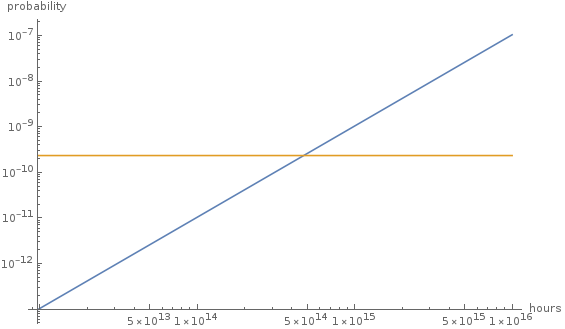
\includegraphics[height=0.25\linewidth]{figures/collision_prob_1mpps_192_bits}
		\label{fig:collisionprob1mpps192bits}
	}
	\subfloat[96 bit nonce, AES-GCM \& ChaCha20]{%
		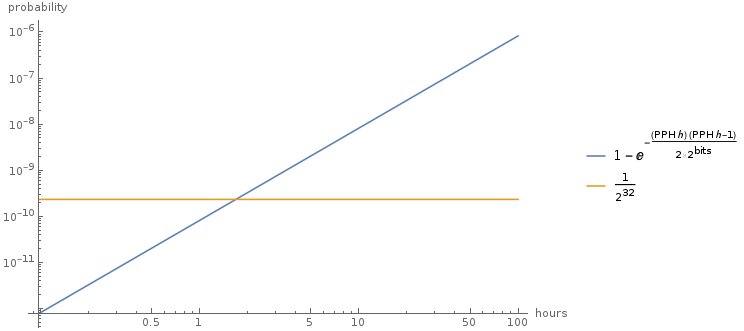
\includegraphics[height=0.25\linewidth]{figures/collision_prob_1mpps_96_bits}
		\label{fig:collisionprob1mpps96bits}
	}
	\caption{Collision probabilities of randomly generated nonces at 1 Mpps}
	\label{fig:collisionprob1mpps}
\end{figure}

%WireGuard protocol specifies IETF chacha20poly1507 with 12 (recheck this) bytes nonces. Since nonce reuse under the same key is devastating for security, implementations have to ensure this never happens. For short nonces it is recommended to increment the previous one, instead of generating random ones.

For 96 bit nonces, like used in AES-GCM (IPsec) and IETF-ChaCha20 (WireGuard), the threshold is passed in under 2 hours of traffic.
This concludes why random generation of small nonces is not recommended. Instead, it is usual to keep the last number and increment it with each packet. In multi-threaded implementations this can become a bottleneck as the nonces are essentially shared state between multiple read-write threads and have to be synchronized.

An possible solution to this problem could be the usage of ciphers with larger nonces, such as XChaCha20. The enlarged value range decreases the probability of collisions over-proportionally, as seen in Figure (b). There it takes $4\times 10^{14}$ hours to reach the same risk level as above. An equivalent of 10 times the age of the sun.

%The following describes different techniques to solve this.
%Note: As an alternative using XChacha20, 192-bit nonce, can be randomly generated, no shared state

%\subsubsection{Mutual exlusive access (atomics, mutex, \texttt{\_\_sync\_add\_and\_fetch()})}
%\subsubsection{One Thread maintains nonces, sends them with work packet}
%\subsubsection{Partitioning}

%\subsubsection{AVX512}
%Intel CPUs throttle frequency if AVX512 (?) code is encountered, this P-state change takes time + the rest of the code runs at slower base frequency.
%Implement this, check freqs, benchmark, see if AVX512 can be worth it.

%


\subsection{Variant 1 - Naive Single Instance}
The first variant is based on the design of OpenVPN and conceptually simple. The whole application consists of a single thread, that completes all tasks of VPN operation.

\begin{figure}[h]
	\centering
	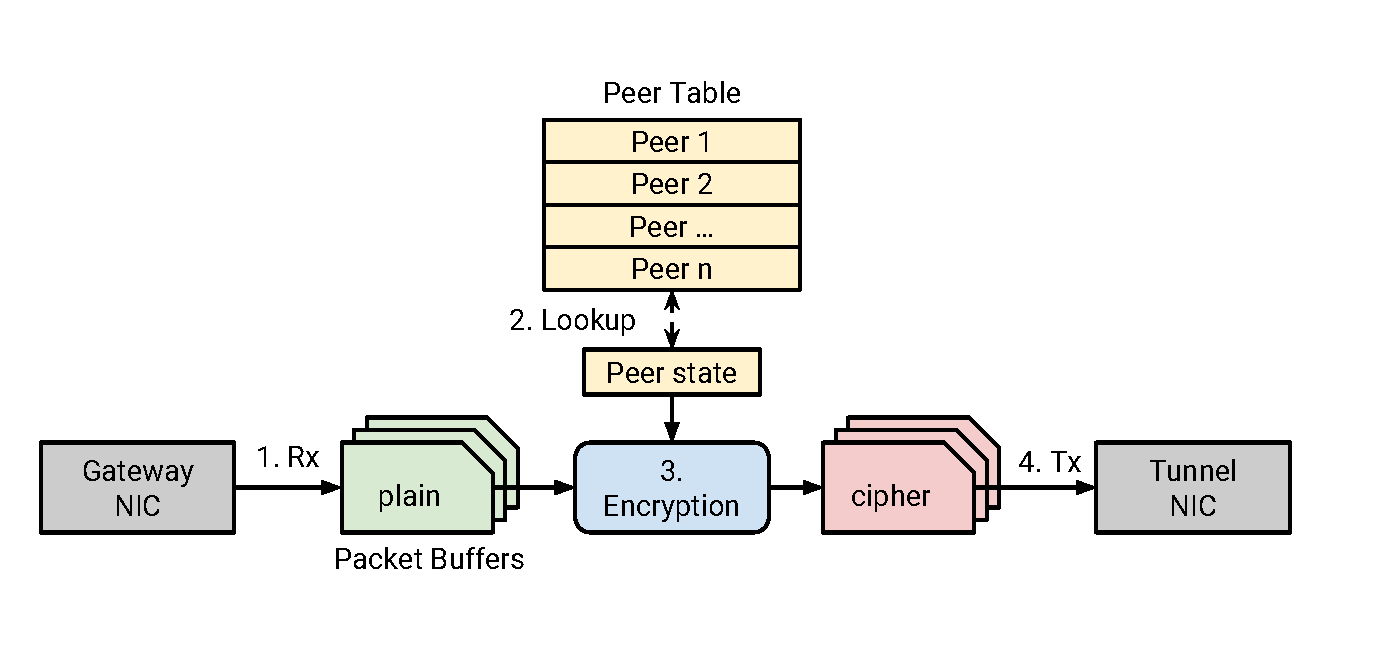
\includegraphics[width=0.9\linewidth]{figures/moonwire-variant-1}
	\caption{Flowchart of MoonWire variant 1}
	\label{fig:moonwire-variant-1}
\end{figure}

In Figure~\ref{fig:moonwire-variant-1} the different steps in the continuous main loop of variant 1 are visualized. The thread starts by receiving incoming packet from the gateway interface in form of a batch of \texttt{rte\_pktbufs}. Each buffer is validated and the associated peer state is looked up in the peer table. If there is a running connection, the buffer is extended, encrypted and new IP headers are inserted. In the last step, all valid packets are send and the remaining ones are freed, thus reclaiming their descriptors and memory into the pool of the gateway.

Due to its single-threaded nature, there is no need for any kind of synchronization on the peer table or state. This simplifies the state-keeping process greatly and poses the least requirements on the used data structures. A simple LPM table such as the one provided by DPDK~\cite{dpdk-lpm-api} can be used to implement the peer table.
This variant does also no suffer from averse traffic pattern, like single-flow traffic. With only one thread, there are no benefits in using RSS and multiple queues. Therefore, uneven packet distribution can not occur. On the contrary, such traffic could even be beneficial, since repeated lookups of the same value utilizes the CPU caches better than different addresses, which generate repeated cache misses and evictions.

On the downside, this variant shares its drawbacks with OpenVPN. Namely, the total lack of horizontal scaling. Other cores can only be utilized by spawning multiple independent instances and fragmenting the routed subnets into smaller chunks.


\subsection{Variant 2 - Independent Workers}
Variant 2 takes the crude scaling attempts necessary for variant 1 or OpenVPN and internalizes them. In summary, this version is most similar to IPsec in the Linux Kernel.

\begin{figure}[h]
	\centering
	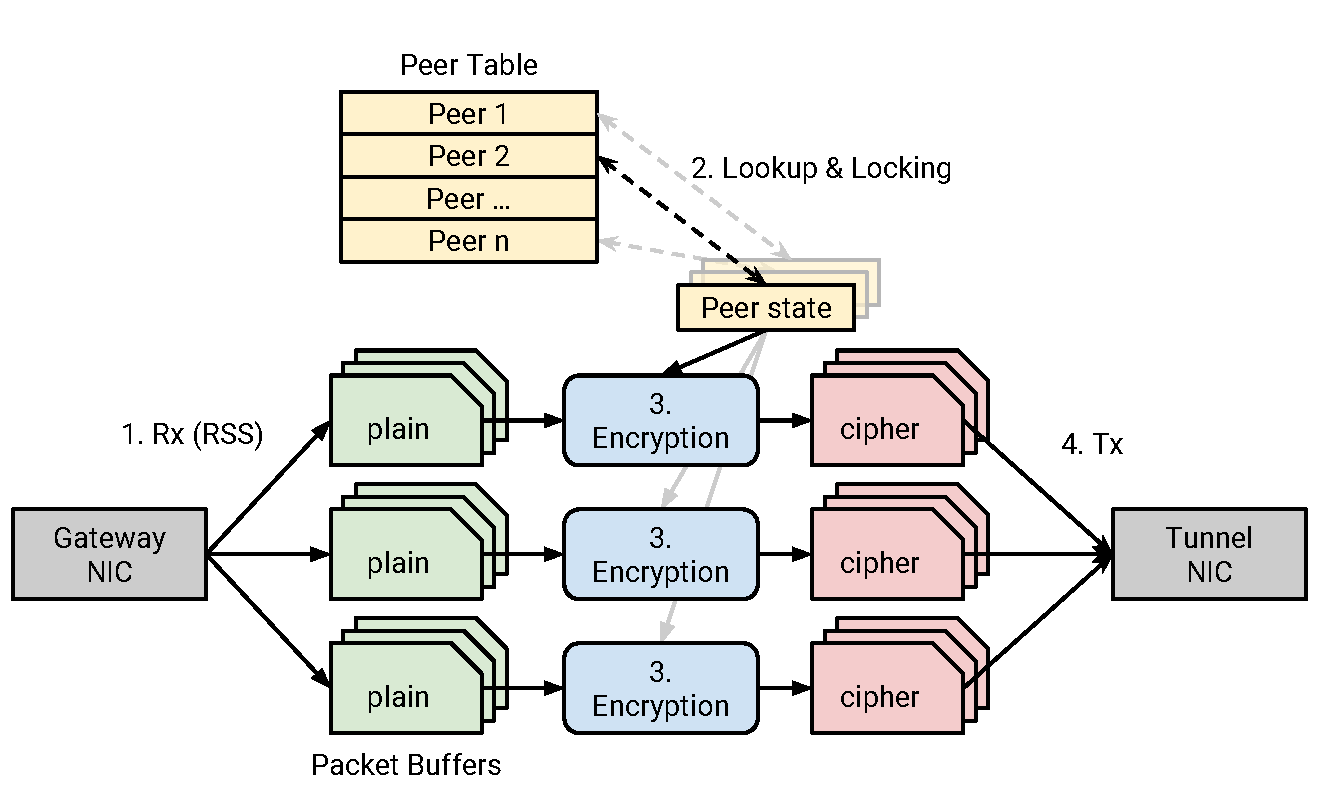
\includegraphics[width=0.9\linewidth]{figures/moonwire-variant-2}
	\caption{Flowchart of MoonWire variant 2}
	\label{fig:moonwire-variant-2}
\end{figure}

As seen in Figure~\ref{fig:moonwire-variant-2}, multiple workers are processing the packets in parallel, each with its own NIC queues. Each worker still completes the whole loop from reception, encryption to transmission. Incoming packets are distributed to multiple queues on the hardware level by the NIC through RSS.
Since there are multiple threads accessing and modifying shared data, data accesses have to be synchronized to prevent corruption. 
The DPDK LPM lookup table is not thread-safe for performance reasons, but read-only lookups can be performed from multiple threads at the same time~\cite{dpdk-fastpath-api}. Fortunately, changes to the table structure are rare, namely when the VPN configuration is modified, so this operation is allowed to be more expensive and slow. 
The peer state, on the other hand, is written to for every packet when the nonce is incremented. In our implementation it is secured by a traditional lock, which a worker thread takes before encrypting an entire batch of packets and releases it afterwards.

There exist many implementations of locks. We take the classic \texttt{pthread\_mutex} from the POSIX threading library and compare it to the \texttt{rte\_spinlock} provided by DPDK, henceforth called variant 2a and 2b respectively. The POSIX mutex internally relies on \texttt{futex} API of the Kernel and is a general purpose lock. In particular, when waiting for a lock to be become free, the calling threads is suspended and does not consume further cycles.
Spinlocks, on the other hand, do not relinquish control to the scheduler, but continuously keep trying. 
This trades latency for energy efficiency, and to some degree performance under heavy contention, as seen in the evaluation~\ref{TODO}.  


\subsection{Variant 3 - Work Pipeline}
In variant 3 the best properties of the previous versions are taken, while avoiding their drawbacks. 
Variant 1 showed, that not utilizing multiple cores will limit performance greatly, as operations like encryption of large buffers inherently need much processing power.
A shared peer state with locks, as implemented in variant 2, inhibits scaling too much, by introducing synchronization overhead, to be viable. 

\begin{figure}[h]
	\centering
	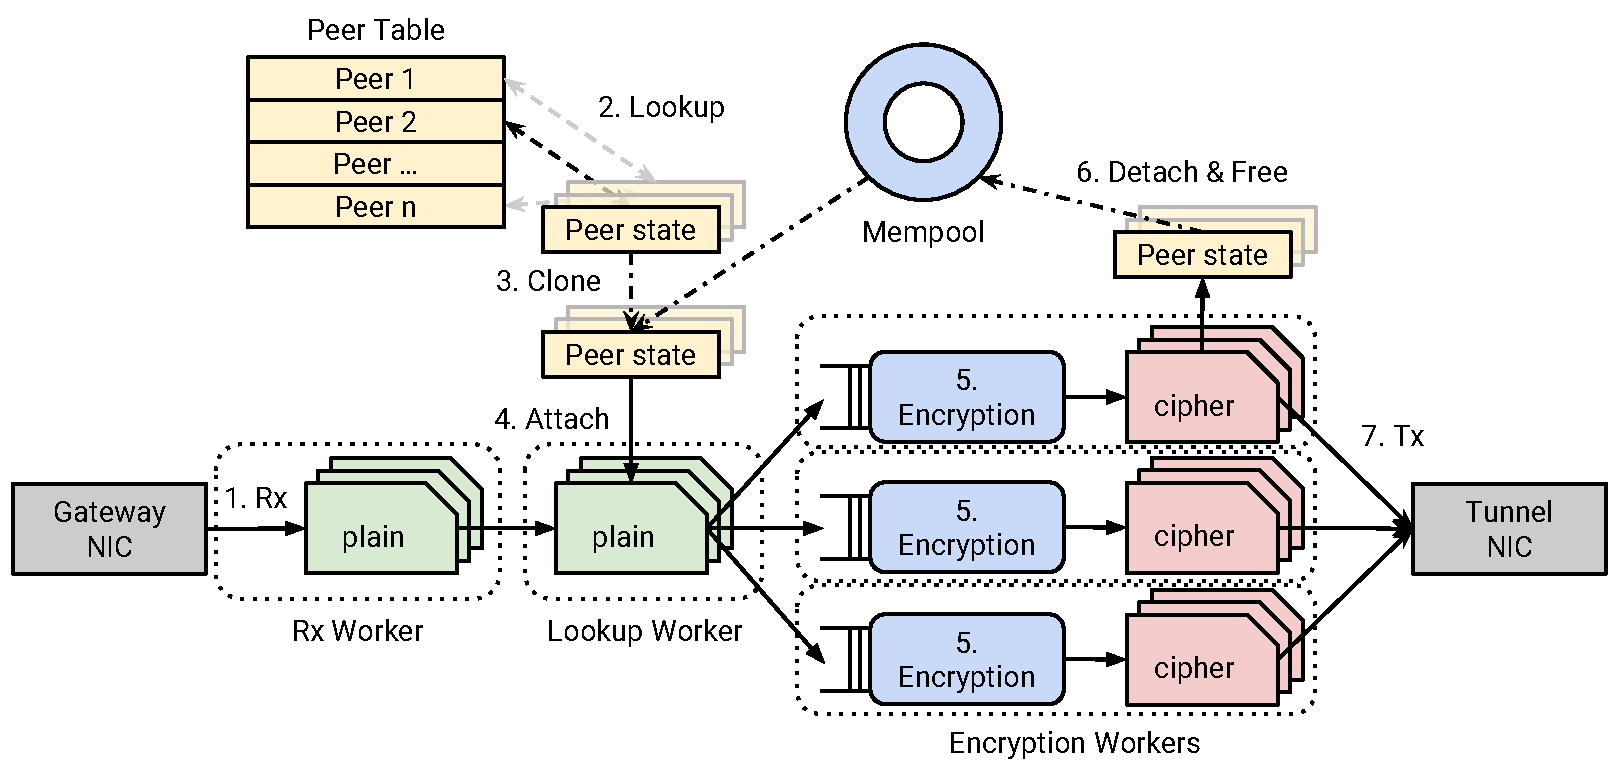
\includegraphics[width=1\linewidth]{figures/moonwire-variant-3}
	\caption{Flowchart of MoonWire variant 3}
	\label{fig:moonwire-variant-3}
\end{figure}

Therefore, a hybrid approach in chosen for variant 3. The peer table and state is still contained in and maintained by a single thread, therefore lock-free, while the encryption stage is parallelized across multiple workers. Instead of handing out mutable peer state references to the workers, the state is cloned and distributed in a message passing manner.
A lookup worker fetches the applicable state to a packet buffer, increments the nonce counter, copies the entire state with all keys and endpoint information into a separate empty buffer, and attaches this buffer to the packet buffer. The \texttt{rte\_membuf} struct includes a member field called \texttt{udata64} for this purpose. The parallel workers now find all information needed for encryption contained in the packet buffer and do not have to updated any shared state.
Since this crypto-args buffer is separate allocated memory, it has to be reclaimed after use. Traditional memory management with \texttt{malloc()/free()} is to slow to be used a million times per second concurrently~\cite{TODO}. Therefore it is implemented the same way as the packet buffers; as fixed-sized, memory-pooled data buffers. 
DPDK exposes the packet buffer memory pools as plain \texttt{rte\_mempools} without the network packet specific customization, so we use them here.

Buffer distribution between the stages happen through DPDK \texttt{rte\_rings}; lock-free, FIFO, high performance queues with batched functions to reduce overhead. 
The step from the lookup to the encryption workers could be solved by having one MPMC queue, but this introduces more shared state than multiple SPSC queues. For one, SPSC semantics allow DPDK to use more relaxed and faster enqueue/dequeue functions without an atomic CMP-XCHG loop~\cite{dpdk-rte-ring-enqueue}. It also reduces false sharing cache evictions caused by dequeues from other workers. Overall this trades memory usage for performance. Distribution over the workers happens in a round-robin fashion to ensure equal load among them.


In a previous version the Rx and the Lookup worker where unified into one. But as shown in Figure~\ref{}, there is a significant amount of time spend for state cloning. To speed this process up, packet reception has been factored out in the final design shown in Figure~\ref{fig:moonwire-variant-3}.


\chapter{Evaluation}
\label{chap:evaluation}

This Chapter evaluates the presented VPN implementations. For this, I firstly define the metrics to measure. ...

The sections about the individual implementations are structured similarly. First we give background information about the protocols and ... . Then we list how the applications are setup for the benchmarks and what configurations we tested. If changes to the test setup were necessary, these are also described there.
Lastly follows the presentations of the results and a detailed analysis of the bottlenecks we could identify. 

\section{Used Hardware and Software Configuration}

\subsubsection{Load Generator}
To generate the required traffic multiple libmoon Lua scripts are used. 

Compared to tools like iperf, this gives us much more control about timings, the exact data send, while also being much more performant. 

By bypassing the Kernel network stack, we can generate any kind or pattern of traffic, without being restricted by security measures or configuration limitations. E.g. it is possible to generate traffic originating from an entire subnet with a single NIC, without having to set any IP address on the interface.

Also it allows the usage of precise rate limits, a topic traditional user-space tools struggle with, as show by \cite{todo}.


%\section{Evaluation of State-of-the-Art VPN Implementations}
\section{Defining Criteria of Performance}


\subsection{Traffic Characteristics}
\subsubsection{Number of Flows}

Pure UDP. UDP is the protocol of choice since it is stateless and does not depend on feedback from the other side. 
It also does not exhibit many side effects TCP has. Correctly benchmarking TCP connections can be difficult and error prone, as TCP has a complicated internal state machine with many configurable variables. It is out of the scope of this thesis to cover the complex interplay of the link MTU, TCP window \& maximum segment sizes (MSS) and scaling algorithms like reno or cubic.

\subsubsection{Packet Rate}
The packet rate describes how many packets per second are processed.

In a benchmark setup we can set a given input rate to the DuT and observe the output rate of the processed packets. 
By increasing the input rate we get a complete picture of how the device behaves under different load conditions.

[Example figure]
Programs seldom scale linearly with the offered load, but exhibit different pattern over the load range. At lower loads the device can handle the all packets, which results in the output rate being equal to the input rate. Resource utilization will be lower than 100\%.

At a certain point this changes as the device enters overload phase and has to drop packets. This does not mean that all resources of the device are fully utilized, but merely that a particular piece has become the bottleneck.
Under overload different patterns can be observed.

\subsubsection{Increasing output}
\subsubsection{Constant output}
\subsubsection{Decreasing output}


\subsubsection{Rate Control Methods}
Packet rate alone does not sufficiently define the traffic pattern. A given target load can be generated by different load-generator methods that, while all delivering the same amount of packets, look different. Figure X shows different configurations. 

\cite{emmerich2015moongen} showed that micro-bursts can have a measurable impact on the DuT. In their tests a Linux Open vSwitch router exhibited a lower interrupt rate for bursty traffic than for CBR traffic.

To verify  that the type for traffic does not overly impact performance of the VPNs, I subjected the DuTs to the different rate-limiting methods. Figures X compare the forwarding rates under varying loads. 

[Figures about rate-limiting]

% TODO
It can be seen that the used method for rate-limiting has very little impact on the forwarding performance of the VPNs. Since the hardware based rate-liming mechanism are more flexible in usage regarding multiple threads, all other benchmarks are performed open-loop with a constant bit rate.

\subsubsection{Packet Size}
Packet size is an important factor in measurements, as clever variation of the sizes allows to gain insights about the inner working of the device under test. This is possible by splitting the costs of handling a packet into two categories. 
The static costs are independent of packets sizes and always occur equally. Things like routing lookups and counters fall into this category: Resolving the destination interface for an IP packet does not depend on the payload if it.
The variable costs on the other hand are heavily influenced by the size and scale accordingly. E.g. en- or decryption only happens to the degree of the bytes there to handle.

By 

Of course, such synthetic traffic pattern do seldom occur in real world usage and might therefore not represent the exact performance numbers. To also gain coverage in this area, I include a second configuration with variable packet sizes. The script sets the size of each packet randomly according to a distribution function. This function has been modeled with data gathered at a uplink of the Deutsches Forschungsnetz (DFN) and is more representative of real world traffic. Figure~\ref{fig:dfn-cdf} shows the probabilities of occurrence for each observed packet size. It can be seen that 27\% of all packets are smaller than 66 bytes and 42\% have the maximum size of 1514 bytes.

\begin{figure}[h]
	\centering
	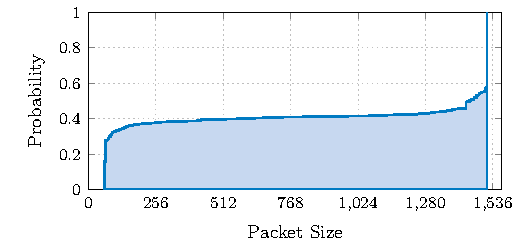
\includegraphics[width=0.9\linewidth]{figures/dfn-cdf}
	\caption{CDF of packet size collected at a DFN Internet uplink}
	\label{fig:dfn-cdf}
\end{figure}

Using these results I conclude that a benchmark should test the static minimum and maximum sizes of 64 and 1518 bytes respectively, as well as a realistic distribution.
 


\subsection{Scenario - Site-to-Site VPN}
\begin{figure}[h]
	\centering
	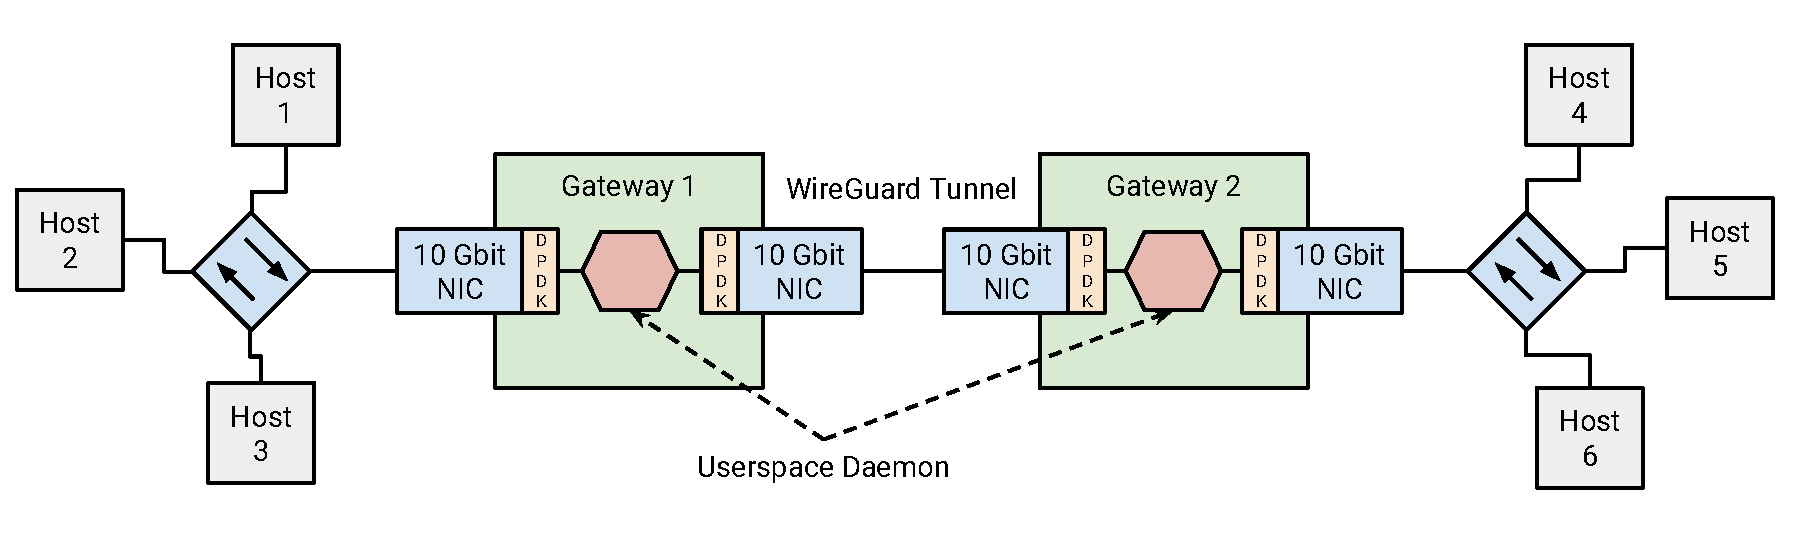
\includegraphics[width=1\linewidth]{figures/PoC-Overview}
	\caption{Overview of Site-to-Site VPN Setup}
	\label{fig:poc-overview}
\end{figure}

%\subsection{Setup B - Many Client Entry Point}

\section{Baseline: Linux  Network Stack \& Router}
With the exception of MoonWire, all three tested VPNs rely on the Kernel network stack for low-level functionality. This includes the handing of drivers, operating the hardware, parsing protocols such as TCP, UDP, IP, queuing and routing of packets.

In benchmarks the costs passing through the network stack is sometimes not separable from the costs of the application.
To classify the performance of the VPNs more accurately, we need some form of baseline performance to determine if a bottleneck is caused by the application or roots in the Linux network stack. Therefore we also measure the performance of it directly.

While others already published performance measurements for Linux~\cite{}, we want comparable values by testing the router and the VPNs against exactly the same traffic patterns, on the same hosts and on the same network equipment. 

\subsection{Forwarding Performance}

Routing is a fundamental operation in a L3 VPN and often offloaded to the Kernel. Before a packet is given to an application by, e.g, virtual interfaces, the Kernel first validates its fields and decides if it is should be further processed.

At some point a packet is given pack to the Linux Kernel, where its destination has to be look
Routing is a fundamental step of the VPN operational process, as all packets have to be validated upon receival and the correct output NIC has to be looked up before sending out encrypted packets.

For the following benchmark we configured one extra route on the DuT, so that it forwards the packets back to the load generator. Including the default gateway to the management host and link scope routes, the main routing table contained six routes.

\begin{figure}[h]
	\centering
	\subfloat[64 byte packets]{%
		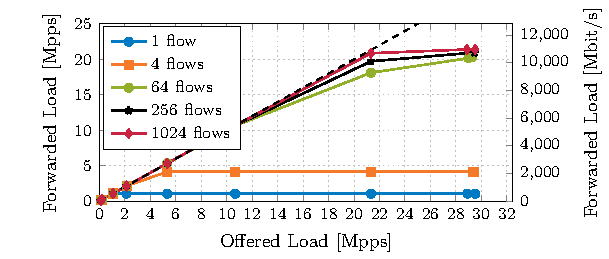
\includegraphics[width=0.5\linewidth]{figures/linux_router_fwd_60_bytes_variable_flows}
		\label{fig:linuxrouterfwd60bytesvariableflows}
	}
	\subfloat[128 byte packets]{%
		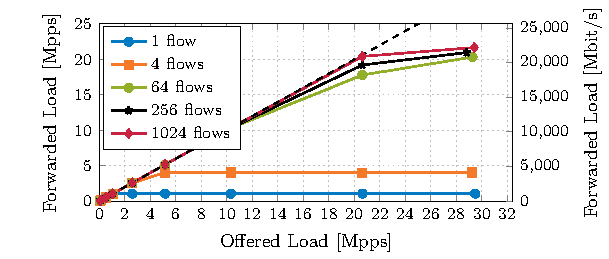
\includegraphics[width=0.5\linewidth]{figures/linux_router_fwd_124_bytes_variable_flows}
\label{fig:linuxrouterfwd124bytesvariableflows}
	}
	
	\subfloat[512 byte packets]{%
		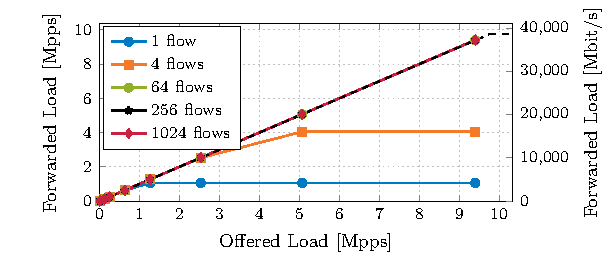
\includegraphics[width=0.5\linewidth]{figures/linux_router_fwd_508_bytes_variable_flows}
\label{fig:linuxrouterfwd508bytesvariableflows}
	}
	\subfloat[1514 byte packets]{%
		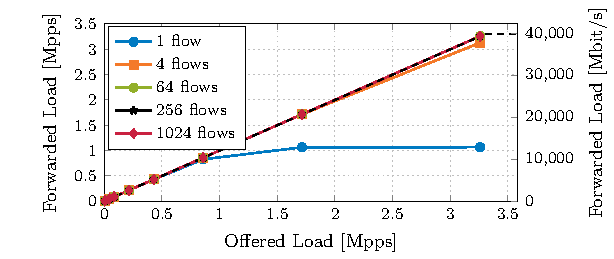
\includegraphics[width=0.5\linewidth]{figures/linux_router_fwd_1510_bytes_variable_flows}
\label{fig:linuxrouterfwd1510bytesvariableflows}
	}
	
	\caption{Linux router forwarding rates with different packet sizes and varying number of flows}
	\label{fig:linux-router-variablebytes-variableflows}
\end{figure}

%TODO DFN traffic pattern

Figure~\ref{fig:linux-router-variablebytes-variableflows} shows the measured rates of the Linux router with traffic of fixed sized packets and a varying number of flows. The dotted line marks the ideal case; each incoming packet is forwarded. 
The x-axes display the applied load to the DuT, while the left and right y-axes measure the traffic, that was received back on the load generator.

It can be seen that the kind of traffic has an measurable impact on the routing level already: traffic consisting of just one or a little number of flows is not as easily processed as traffic with many flows. For a single flow of 64 bytes the forwarding rate is at best 1.006 Mpps, while with 1024 flows it increases steadily to around 21.3 Mpps. 
Although the forwarding rates plateau at a certain level, they do not decrease after that. This means this system is not susceptible to a trivial DoS attack where an attacker just sends millions of packets to lower performance for everyone else.

The influence of packet size is twofold. One the one hand it does not decrease the rate of which packets are processed. Traffic of four flows always peaks at 4 Mpps. On the other hand it naturally increases the throughput in terms of bytes per second. So can the link bandwidth of 40 Gbit/s be reached with 512 byte packets and 64 flows.

This is somewhat expected for a router, as it only looks at the first few bytes in the Ethernet and IP header of a packet to make its routing decision. Figure~\ref{fig:linux-router-cycles} fortifies this observation.

Overall it can be said that the Linux network stack is able to handle 10G links, if either the packets are not very small or a sufficient number of flows run in parallel.

\begin{figure}[h!]
	\centering
	\subfloat[Cycles per packet]{%
		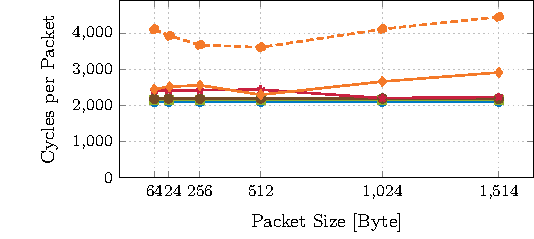
\includegraphics[width=0.7\linewidth]{figures/linux-cycles-per-packet}
		\label{fig:linux-cycles-per-packet}
	}
	
	\subfloat[Cycles per byte]{%
		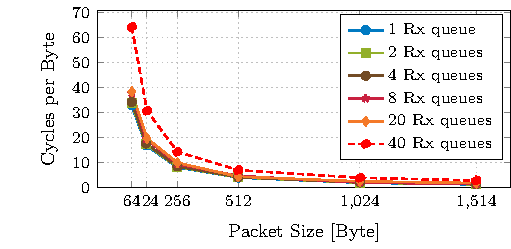
\includegraphics[width=0.7\linewidth]{figures/linux-cycles-per-byte}
		\label{fig:linux-cycles-per-byte}
	}
	
	\caption{Cycle spend for Linux routing \& forwarding}
	\label{fig:linux-router-cycles}
\end{figure}


\subsection{Packet Distribution}
The first step to investigate the slow forwarding performance with traffic consisting of few flows is to look at the CPU utilization of the DuT. This can be done with the \texttt{perf} toolset which includes a sampling profiler. By comparing the values read from the CPU internal performance \& cycle counters to the clock rate of the CPU, we can calculate the relative utilization of each core:

\begin{equation}\label{eq-cpu}
\dfrac{\mathrm{recorded\ cycles}}{\mathrm{runtime}} \times \dfrac{1}{\mathrm{CPU\ clock\ rate}} = \mathrm{CPU\ utilization}
\end{equation}

%System wide measurement. cycles, perf

\begin{figure}[h]
	\centering
	\subfloat[1 flow]{%
		\resizebox{0.33\columnwidth}{!}{%
			\begin{tabular}[htp]{|c|c|c|c|c|}%
\hline
\cellcolor{TUMBlue!0} CPU0 & \cellcolor{TUMBlue!0} CPU1 & \cellcolor{TUMBlue!0} CPU2 & \cellcolor{TUMBlue!0} CPU3 & \cellcolor{TUMBlue!93} CPU4 \\
\hline
\cellcolor{TUMBlue!0} CPU5 & \cellcolor{TUMBlue!0} CPU6 & \cellcolor{TUMBlue!0} CPU7 & \cellcolor{TUMBlue!0} CPU8 & \cellcolor{TUMBlue!0} CPU9 \\
\hline
\cellcolor{TUMBlue!0} CPU10 & \cellcolor{TUMBlue!0} CPU11 & \cellcolor{TUMBlue!0} CPU12 & \cellcolor{TUMBlue!0} CPU13 & \cellcolor{TUMBlue!6} CPU14 \\
\hline
\cellcolor{TUMBlue!0} CPU15 & \cellcolor{TUMBlue!0} CPU16 & \cellcolor{TUMBlue!3} CPU17 & \cellcolor{TUMBlue!0} CPU18 & \cellcolor{TUMBlue!0} CPU19 \\
\hline
\cellcolor{TUMBlue!0} CPU20 & \cellcolor{TUMBlue!0} CPU21 & \cellcolor{TUMBlue!0} CPU22 & \cellcolor{TUMBlue!0} CPU23 & \cellcolor{TUMBlue!0} CPU24 \\
\hline
\cellcolor{TUMBlue!0} CPU25 & \cellcolor{TUMBlue!0} CPU26 & \cellcolor{TUMBlue!0} CPU27 & \cellcolor{TUMBlue!0} CPU28 & \cellcolor{TUMBlue!0} CPU29 \\
\hline
\cellcolor{TUMBlue!0} CPU30 & \cellcolor{TUMBlue!0} CPU31 & \cellcolor{TUMBlue!0} CPU32 & \cellcolor{TUMBlue!0} CPU33 & \cellcolor{TUMBlue!0} CPU34 \\
\hline
\cellcolor{TUMBlue!2} CPU35 & \cellcolor{TUMBlue!0} CPU36 & \cellcolor{TUMBlue!0} CPU37 & \cellcolor{TUMBlue!0} CPU38 & \cellcolor{TUMBlue!0} CPU39 \\
\hline
			\end{tabular}
		}
	}
	%\hfill
	\subfloat[4 flows]{%
		\resizebox{0.33\columnwidth}{!}{%
			\begin{tabular}[htp]{|c|c|c|c|c|}%
\hline
\cellcolor{TUMBlue!1} CPU0 & \cellcolor{TUMBlue!0} CPU1 & \cellcolor{TUMBlue!0} CPU2 & \cellcolor{TUMBlue!0} CPU3 & \cellcolor{TUMBlue!92} CPU4 \\
\hline
\cellcolor{TUMBlue!0} CPU5 & \cellcolor{TUMBlue!0} CPU6 & \cellcolor{TUMBlue!0} CPU7 & \cellcolor{TUMBlue!0} CPU8 & \cellcolor{TUMBlue!0} CPU9 \\
\hline
\cellcolor{TUMBlue!0} CPU10 & \cellcolor{TUMBlue!0} CPU11 & \cellcolor{TUMBlue!0} CPU12 & \cellcolor{TUMBlue!0} CPU13 & \cellcolor{TUMBlue!92} CPU14 \\
\hline
\cellcolor{TUMBlue!0} CPU15 & \cellcolor{TUMBlue!0} CPU16 & \cellcolor{TUMBlue!0} CPU17 & \cellcolor{TUMBlue!0} CPU18 & \cellcolor{TUMBlue!0} CPU19 \\
\hline
\cellcolor{TUMBlue!0} CPU20 & \cellcolor{TUMBlue!92} CPU21 & \cellcolor{TUMBlue!0} CPU22 & \cellcolor{TUMBlue!0} CPU23 & \cellcolor{TUMBlue!0} CPU24 \\
\hline
\cellcolor{TUMBlue!0} CPU25 & \cellcolor{TUMBlue!0} CPU26 & \cellcolor{TUMBlue!0} CPU27 & \cellcolor{TUMBlue!0} CPU28 & \cellcolor{TUMBlue!0} CPU29 \\
\hline
\cellcolor{TUMBlue!0} CPU30 & \cellcolor{TUMBlue!92} CPU31 & \cellcolor{TUMBlue!0} CPU32 & \cellcolor{TUMBlue!2} CPU33 & \cellcolor{TUMBlue!0} CPU34 \\
\hline
\cellcolor{TUMBlue!0} CPU35 & \cellcolor{TUMBlue!1} CPU36 & \cellcolor{TUMBlue!0} CPU37 & \cellcolor{TUMBlue!0} CPU38 & \cellcolor{TUMBlue!0} CPU39 \\
\hline
			\end{tabular}
		}
	}
	
	\subfloat[64 flows]{%
		\resizebox{0.33\columnwidth}{!}{%
			\begin{tabular}[htp]{|c|c|c|c|c|}%
\hline
\cellcolor{TUMBlue!93} CPU0 & \cellcolor{TUMBlue!93} CPU1 & \cellcolor{TUMBlue!93} CPU2 & \cellcolor{TUMBlue!88} CPU3 & \cellcolor{TUMBlue!93} CPU4 \\
\hline
\cellcolor{TUMBlue!67} CPU5 & \cellcolor{TUMBlue!93} CPU6 & \cellcolor{TUMBlue!93} CPU7 & \cellcolor{TUMBlue!93} CPU8 & \cellcolor{TUMBlue!74} CPU9 \\
\hline
\cellcolor{TUMBlue!0} CPU10 & \cellcolor{TUMBlue!61} CPU11 & \cellcolor{TUMBlue!0} CPU12 & \cellcolor{TUMBlue!69} CPU13 & \cellcolor{TUMBlue!93} CPU14 \\
\hline
\cellcolor{TUMBlue!0} CPU15 & \cellcolor{TUMBlue!0} CPU16 & \cellcolor{TUMBlue!0} CPU17 & \cellcolor{TUMBlue!39} CPU18 & \cellcolor{TUMBlue!69} CPU19 \\
\hline
\cellcolor{TUMBlue!73} CPU20 & \cellcolor{TUMBlue!73} CPU21 & \cellcolor{TUMBlue!73} CPU22 & \cellcolor{TUMBlue!0} CPU23 & \cellcolor{TUMBlue!93} CPU24 \\
\hline
\cellcolor{TUMBlue!65} CPU25 & \cellcolor{TUMBlue!73} CPU26 & \cellcolor{TUMBlue!93} CPU27 & \cellcolor{TUMBlue!73} CPU28 & \cellcolor{TUMBlue!93} CPU29 \\
\hline
\cellcolor{TUMBlue!76} CPU30 & \cellcolor{TUMBlue!61} CPU31 & \cellcolor{TUMBlue!76} CPU32 & \cellcolor{TUMBlue!93} CPU33 & \cellcolor{TUMBlue!93} CPU34 \\
\hline
\cellcolor{TUMBlue!77} CPU35 & \cellcolor{TUMBlue!93} CPU36 & \cellcolor{TUMBlue!93} CPU37 & \cellcolor{TUMBlue!0} CPU38 & \cellcolor{TUMBlue!93} CPU39 \\
\hline
			\end{tabular}
		}
	}
	\subfloat[256 flows]{%
		\resizebox{0.33\columnwidth}{!}{%
			\begin{tabular}[htp]{|c|c|c|c|c|}%
\hline
\cellcolor{TUMBlue!89} CPU0 & \cellcolor{TUMBlue!93} CPU1 & \cellcolor{TUMBlue!93} CPU2 & \cellcolor{TUMBlue!93} CPU3 & \cellcolor{TUMBlue!93} CPU4 \\
\hline
\cellcolor{TUMBlue!91} CPU5 & \cellcolor{TUMBlue!93} CPU6 & \cellcolor{TUMBlue!93} CPU7 & \cellcolor{TUMBlue!88} CPU8 & \cellcolor{TUMBlue!46} CPU9 \\
\hline
\cellcolor{TUMBlue!60} CPU10 & \cellcolor{TUMBlue!90} CPU11 & \cellcolor{TUMBlue!90} CPU12 & \cellcolor{TUMBlue!90} CPU13 & \cellcolor{TUMBlue!93} CPU14 \\
\hline
\cellcolor{TUMBlue!42} CPU15 & \cellcolor{TUMBlue!90} CPU16 & \cellcolor{TUMBlue!75} CPU17 & \cellcolor{TUMBlue!59} CPU18 & \cellcolor{TUMBlue!60} CPU19 \\
\hline
\cellcolor{TUMBlue!62} CPU20 & \cellcolor{TUMBlue!93} CPU21 & \cellcolor{TUMBlue!62} CPU22 & \cellcolor{TUMBlue!91} CPU23 & \cellcolor{TUMBlue!93} CPU24 \\
\hline
\cellcolor{TUMBlue!92} CPU25 & \cellcolor{TUMBlue!93} CPU26 & \cellcolor{TUMBlue!93} CPU27 & \cellcolor{TUMBlue!77} CPU28 & \cellcolor{TUMBlue!93} CPU29 \\
\hline
\cellcolor{TUMBlue!91} CPU30 & \cellcolor{TUMBlue!93} CPU31 & \cellcolor{TUMBlue!93} CPU32 & \cellcolor{TUMBlue!93} CPU33 & \cellcolor{TUMBlue!93} CPU34 \\
\hline
\cellcolor{TUMBlue!84} CPU35 & \cellcolor{TUMBlue!93} CPU36 & \cellcolor{TUMBlue!92} CPU37 & \cellcolor{TUMBlue!89} CPU38 & \cellcolor{TUMBlue!93} CPU39 \\
\hline
			\end{tabular}
		}
	}
	\caption{CPU utilization of the Linux router during peak load}
	\label{fig:linux-router-60bytes-heatmap}
\end{figure}


Figures~\ref{fig:linux-router-60bytes-heatmap} (a) to (d) show heatmaps of the CPU utilization per core for the different traffic pattern. The snapshots are taken at peak forwarding rate for the respective kind of traffic.

For the single-flow traffic it can be seen that only one core, in this case CPU 4, is actually processing incoming packets, while the others are effectively idle.
This explains the much lower forwarding rate compared to the other traffic, one core can simply not keep up with the amount of packets. 
Compared to traffic with, e.g. 256 flows, the trend line becomes clear. More parallel flows result in a more distributed load, as seen in Figure (d), where all cores are utilized to some degree and a much higher forwarding rate can be achieved.

As explained in Section\ref{}, the NIC uses a hash function over the packet header to distribute incoming packets to the Rx-queues in a technique called receive-side scaling (RSS). If each header contains the same values, as it is the case for single-flow traffic, all packets end up in the same queue, negating any possible scaling effects. This is further worsened by the default configuration of how the queues are serviced by the CPUs. On symmetric multi-processor (SMP) systems the Kernel configures as many queues as there are CPU cores and binds them 1:1. Each core then only receives interrupts for exactly one Rx-queue. The binding, called IRQ-affinity\cite{}, can be checked and configured via the \texttt{sysfs} pseudo filesystem under \texttt{/proc/irq} and \texttt{/proc/interrupts}.

\subsubsection{Alternative IRQ/Queue Configurations}
Apart from the default 1:1 mapping, there exist other possible configurations.
Generally, there is advise against delivering one interrupt to multiple CPUs as it can decrease performance due to caching effects~\cite{}.
However, in the case of single-flow traffic a round-robin distribution over multiple cores could still have a net benefit. Listing~\ref{lst:alt-irq} shows how to configure a single rx-queue that delivers interrupts to the CPUs 0 to 7.

\begin{lstlisting}[caption={Commands to configure a single RXTX queue and bind it to multiple cores},captionpos=b,label={lst:alt-irq}]
ethtool -L eth0 combined 1;
echo 0-7 > /proc/irq/124/smp_affinity_list
\end{lstlisting}

Linux also provides Transmit Packet Steering (XPS) as a means to control the CPU-to-queue mapping on transmit path. Under the sysfs directories \texttt{/sys/class/net/<dev>/queues/tx-<n>/xps\_cpus} it is possible to define which CPUs 

On our testbed hardware this did not work, as the NIC still delivered interrupts to the first CPU of the affinity list only.

Another approach is to reduce the number of queues, with the goal to improve efficiency. In Section~\ref{sec:linux-code-analysis} we try this approach and show, that it can reduce lock contention.

\subsection{Source Code Analysis: Spinlocks}
\label{sec:linux-code-analysis}
We also record which tasks the CPUs perform to see where the cycles are spend. Graph X displays the detailed workload grouped into major categories.
In cases of uneven load distribution we pick a core with a high load. 

\begin{table}
	\centering
	\resizebox{0.5\linewidth}{!}{
		\begin{tabular}{rl}
			\toprule
			Percentage & Symbol \\
			\midrule
 19.39\% & [k] \_raw\_spin\_lock\\
10.07\% & [k] fib\_table\_lookup\\
5.73\% & [k] i40e\_lan\_xmit\_frame\\
5.16\% & [k] i40e\_napi\_poll\\
4.02\% & [k] ip\_finish\_output2\\
2.75\% & [k] ip\_route\_input\_noref\\
2.66\% & [k] \_\_slab\_free\\
2.43\% & [k] \_\_build\_skb\\
2.26\% & [k] \_\_netif\_receive\_skb\_core\\
2.19\% & [k] kmem\_cache\_alloc\\
%2.18\% & [k] dev\_gro\_receive\\
%2.06\% & [k] ip\_rcv\\
%1.98\% & [k] \_\_netdev\_alloc\_skb\\
%1.92\% & [k] udp\_v4\_early\_demux\\
%1.90\% & [k] \_\_dev\_queue\_xmit\\
%1.78\% & [k] ip\_forward\\
%1.74\% & [k] fib\_validate\_source\\
%1.60\% & [k] \_\_local\_bh\_enable\_ip\\
%1.45\% & [k] cmpxchg\_double\_slab.isra.54\\
			\bottomrule
		\end{tabular}
	}
	\caption{Top 10 most cycle consuming functions in Linux router with 4 queues}
	\label{tab:linux-stacktrace}
\end{table}

\subsubsection{Spinlock in Tx Path}
Entry: https://elixir.bootlin.com/linux/v4.4.109/source/net/core/dev.c\#L3112
Calls, since NICs have queues: https://elixir.bootlin.com/linux/v4.4.109/source/net/core/dev.c\#L2939
Has a per queue spinlock taken per skb send

Commit that improved perf: https://github.com/torvalds/linux/commit/79640a4ca6955e3ebdb7038508fa7a0cd7fa5527

It can be seen that a large portion of the time is spend in synchronization functions.
Synchronization often behaves differently depending on the number of participants. E.g. the performance of a mutex scales inversely with number of threads competing for it~\cite{}. To get a better understanding of this area, we measure the cycles spend synchronizing while controlling the number of cores active.
One could craft sophisticated traffic with flows that would exactly utilize the wanted cores, but this is unreliable and rather complicated. It is easier to configure the number of RX queues of the NIC directly. On Linux this can be done with ethtool~\cite{}:

\begin{lstlisting}[caption={Command to configure 8 RXTX queues on a NIC},captionpos=b,label={lst:include-fix}]
ethtool -L eth0 combined 8
\end{lstlisting}

Further, traffic with many flows should be used so that all queues get equally utilized and uneven load does not occur.

[Graph: detailed CPU loads vs. \#queues]
\begin{figure}[h]
	\centering
	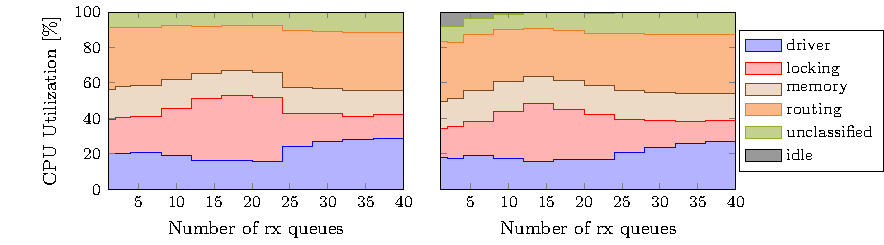
\includegraphics[width=1\linewidth]{figures/linux_spinlock_60_bytes}
	\caption{}
	\label{fig:linuxspinlock60bytes}
\end{figure}



In Figure X it can be seen that the synchronization share indeed increases with the number of queues, and therefore cores, active. This also explains the less-than-linear scaling effect when adding more queues. Time spend in spinlocks is not used to process packets, thus leading to a lower per-core forwarding rate with more cores. This is shown in Figure X.


Overall the performance of the Linux Kernel is comparably good. A 10 Gbit link filled with minimally sized packets can be fully handled by X cores. One should keep in mind, that these benchmarks are not fully illustrative of the capabilities of Linux as a router, but only serve as a baseline for our other measurements. A real world router has large routing tables and many NICs, while our setup only consists of two subnets and two NICs.

\section{IPsec}

IPsec is an IETF standard for network layer security in IP networks.

Engineered to academic perfection, layered approach, key exchange completely separate
Very complex to run/configure correctly. 

As part of this Thesis I will evaluate the IPsec implementation of the Linux Kernel. 
Only the en- and decryption are studied, as the key exchange mechanism are not relevant in throughput evaluations. They can have an impact on the latency of the initial packet, but do later only run as part of re-keying operations. Therefore I have refrained from using a complete IPsec software suite like strongSwan or X, and configured the devices directly with static keys using the iproute2 tools. Table~\ref{tab:ipsec-config} shows the exact settings.

RFC4543 GCM (AES-GMAC) is an esp aead cipher, but does not encrypt the payload. 
\url{https://tools.ietf.org/html/rfc4543#section-2}

\begin{table}[h]
	\centering
	\begin{tabular}{r c c c}
		\# & Configuration & Cipher & Auth \\ 
		\hline 
		1 & ESP tunnel mode & RFC4106 AES-GCM & AEAD\\
		2 & ESP tunnel mode & AES-128-CBC & HMAC-SHA-256 \\
		3 & ESP tunnel mode & none & HMAC-SHA-256 \\
		4 & ESP tunnel mode & none & none\\
	\end{tabular}
	\caption{Tested IPsec configurations}
	\label{tab:ipsec-config}
\end{table}

\begin{lstlisting}[caption={iproute2 command to create a SP on the gateway host},captionpos=b,label={lst:create-SP}]
ip xfrm policy add \
	dir out \
	src 10.0.0.0/16 dst 10.2.0.0/16 \
	tmpl src 10.1.0.1 dst 10.1.0.2 \
	proto esp mode tunnel
\end{lstlisting}


xfrm (transform) layer
Code runs as part of software interrupt handler (ksoftirqd). Softirq runs on same core has the original hardware interrupt.
bound to the core handling the interrupt

\subsection{Encryption: Boundedness to NIC queues \& Multi-core Scaling}
Incoming packets are handled on the same core that received it from the NIC queue. 
There is no distribution step, encryption happens as part of the forwarding step.
Queue -> core mapping can be configured, default is 1:1

[graph: forward rate vs \#flows]

[heatmap: CPU util vs. \#flows]

[graph with spinlock\% vs cores]
[graph: forward rate per core vs flows at 100\% load]
TODO: reduce \# of queues (ethtool), seems to improve perf

TODO: change number of rx descriptors, looks like no impact

TODO: effects of spreading the interrupts N:N

\subsubsection{Different Ciphers}
[graph: compare null cipher with aead]

\subsubsection{Effects of Packet Sizes}
[graph: many flow setup - mpps vs packet size]
[graph: cpu load - encryption functions should be higher]

Calculate metrics like cycles per byte


\subsection{Scaling through Multiple Security Associations}
In Figure X it can be seen that a lot of time is spend synchronizing access to data structures. One such data structure is the IPsec security association (SA) which defines how a packet should be handled. In the Linux Kernel a SA is represented by the \texttt{struct xfrm\_state}~\cite{linux-xfrm-struct}. Among other configuration it contains the replay protection information and a spinlock to synchronize access. 

To enable the detection of duplicate packets on the receiving side, each processed packet gets an incrementing sequence number, which is stored in the IPsec AH header. 
% This number is set as part of the output step of the xfrm framework before a packet is send. 
Since multiple CPUs can process packets governed by the same SA in parallel, each CPU first has to acquire the spinlock to the \texttt{xfrm\_state} before it can modify it. This happens in the \texttt{xfrm\_output\_one()} function~\cite{linux-xfrm-output}, which in turn calls the \texttt{xfrm\_replay\_overflow()} function~\cite{linux-xfrm-replay-overflow} to increment and read the current output sequence number (\texttt{replay.oseq}).
In summary this means, that with only a single SA a de-facto global spinlock has to be acquired and released for each packet, contributing to the slow forwarding rates compared to the baseline measurement.

To distribute this contention over multiple locks, additional SAs can be set up. Each SA then only handles a small subset of the traffic by restricting it to, e.g., a single source IP address, as show in line 6 of Listing~\ref{lst:create-multi-sa}.

\begin{lstlisting}[caption={iproute2 command to create 128 SAs},captionpos=b,label={lst:create-multi-sa}]
for SUBNET in $(seq 2 1 128)
do
	ip xfrm state add \
		src 10.1.0.1 dst 10.1.0.2 \
		proto esp spi 0x$SUBNET mode tunnel enc "ecb(cipher_null)" "" \
		sel src 10.0.0.$SUBNET/32
done
\end{lstlisting}

%TODO Graph
\begin{figure}[h]
	\centering
	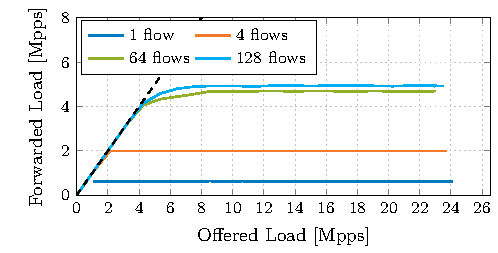
\includegraphics[width=0.7\linewidth]{figures/ipsec_multi_sa_no_cipher_fwd_60_bytes_variable_flows}
	\caption{IPsec forwarding rate with 128 SAs and null cipher}
	\label{fig:ipsecmultisafwd60bytesvariableflows}
\end{figure}

Figure~\ref{fig:ipsecmultisafwd60bytesvariableflows} shows the results of this optimization.


[CPU load graph]
\subsection{Decryption: CPU Clock Rate}

\section{OpenVPN}

OpenVPN is a cross-platform, open source VPN suite. It defines its own protocol 

pure userspace, cross-platform, very modular and configurable
relies on crypto-lib for crypto (openssl)
single-threaded, (e)poll/kqueue/select for socket multiplexing
optional scaling through processes,

\subsection{Tested Configuration}

%Custom openvpn build, v2.4.6, ./configure --disable-ssl --disable-lzo --disable-plugin-auth-pam CFLAGS='-g -O2 -fno-omit-frame-pointer'
%TODO: vergleich ohne debug flags

The only OpenVPN binary supplied by the distributions package manager was an optimized build without debugging symbols. To get more detailed stack traces and resolved function names in our measurements, we build our own binary with the flags shown in Line~19 of Listing~\ref{lst:openvpn-prep}. The remaining preparation steps for the DuT are also given there. In a preliminary test between the distributed and our version, we could not find a performance difference. The OpenVPN version build is 2.4.6 with OpenSSL 1.0.2g as backend.

We configured OpenVPN in L3 tunnel mode with TUN devices, since this implements our site-to-site scenario. Following common practice, packets are delivered over UDP, because it is faster than TCP and avoids problems with window sizes and packet reordering. The exact configuration can be found in Listing~\ref{lst:openvpn-setup}.

%TUN, because faster
%UDP, faster
%point-to-point,
%static key, simpler, no impact after handshake

For the cryptographic parameters we choose ciphers that match the ones used in IPsec and WireGuard most closely. ChaCha20 or AES-GCM is not available, therefore AES-CBC takes it place. While OpnVPN supports much greater number of ciphers and digest algorithms, most of them have been broken~\cite{} or are deemed insecure~\cite{} and are not further studied. The high configurability of OpenVPN allows selective application of encryption, authentication and even replay protection.
In Table~\ref{tab:openvpn-cipher-matrix} all tested combinations are listed.

\begin{lstlisting}[caption={DuT peraration steps for OpenVPN},captionpos=b,label={lst:openvpn-prep},language=bash]
echo 1 > /sys/devices/system/cpu/intel_pstate/no_turbo
IF1=ens3f0
IF2=ens4f0
ip addr flush dev $IF1
ip addr flush dev $IF2
ip a add 10.0.0.1/16 dev $IF1
ip a add 10.1.0.1/24 dev $IF2
ip l set mtu 1600 dev $IF1
ip l set mtu 1600 dev $IF2
ip l set up dev $IF1
ip l set up dev $IF2
sysctl -w net.ipv4.ip_forward=1
arp -s 10.1.0.2 68:05:CA:32:44:98

# build openvpn, debug and clean version
pushd ~
wget https://swupdate.openvpn.org/community/releases/openvpn-2.4.6.tar.gz
tar -xf openvpn-2.4.6.tar.gz
cd openvpn-2.4.6
./configure --disable-ssl --disable-lzo --disable-plugin-auth-pam CFLAGS='-g -O2 -fno-omit-frame-pointer'
make -j && make install

cat << EOF > ~/static.key
-----BEGIN OpenVPN Static key V1-----
69fb86b7243dc8ce3d6647d3dcbc1026
...
-----END OpenVPN Static key V1-----
EOF
\end{lstlisting}


\begin{lstlisting}[caption={OpenVPN command for setup 1 on the DuT},captionpos=b,label={lst:openvpn-setup}]
openvpn --verb 3 \
	 --dev tun --proto udp \
	 --local 10.1.0.1 --remote 10.1.0.2 \
	 --route 10.2.0.0 255.255.0.0 --ifconfig 192.168.0.1 192.168.0.2 \
	 --cipher AES-256-CBC --auth SHA256 --secret /etc/openvpn/static.key
\end{lstlisting}

\begin{table}
	\centering
	\begin{tabular}[htp]{lccc}
		\toprule
		\# & Cipher & Auth & Replay Protection\\
		\midrule
		1 & AES-256-CBC & HMAC-SHA256 & yes \\
		2 & AES-128-CBC & HMAC-SHA256 & yes \\
		3 & AES-128-CBC & none & yes \\
		4 & none & none & no \\
		\bottomrule
	\end{tabular}
	\caption{Tested OpenVPN configurations}
	\label{tab:openvpn-cipher-matrix}
\end{table}

\subsection{Results and Analysis}

% [graph: forwarding rates vs. load]

%TODO: intro

Figures~\ref{fig:openvpn-setup1-variablebytes-variableflows} (a) to (d) show how OpenVPN setup 1 behaves under increasing load of packets with fixed size. Each graph contains the results for a specific packet size and different number of flows. 
The bottom and top x-axes show the offered load in Mpps and Mbit/s respectively, while left and right y-axes show the processed load.

Firstly, it is evident, that the forwarded rate is not very high independent of the kind of offered traffic. It is highest for 64 byte packets at 0.XX Mpps

Another point worth noting is, that the number of flows in the traffic only has a small impact on the performance of OpenVPN. The rates vary very little at a given load and follow the same trend as the load increases. This seems different from what we observed in the baseline benchmark, but can be explained by the low amount of packets per second. The Linux router starts dropping packets at 1.X Mpps for single-flow traffic, while OpenVPN generally processes only a fraction of this. This rules out the router as a limiting factor. If it were, the rates for 256 and 1024 flows should be higher.

Lastly, we found a repeating pattern that is independent of the packet sizes but only occurs with a high number of flows. From 0 Mpps to 0.12 Mpps the application processes each packet without dropping any. After that it can not keep up with the demand and stays nearly stable up to around 0.5 Mpps load. Then it breaks in drastically and stops forwarding at 1 Mpps load. 
This can be explained by looking at the DuT's CPU utilization at a per-CPU level during the runs. In the heatmap in Figure~\ref{fig:openvpn-setup1-60bytes-heatmap} this is visualized through the shading of each field. The higher the load on a core was, the more intense it is colored. For one flow we see two utilized cores, one doing the network stack operations as in the baseline benchmark and one core for the single-thread OpenVPN process, as expected. But as the number of flows increases, more cores start serving NIC queues and the OS is pressured to find a free CPU for the OpenVPN user-space application. The Linux scheduler by default prioritizes user-space processes lower than IRQ handlers, therefore it will not schedule the VPN process under overload, resulting in the observed 0 Mpps processing rate. In the next paragraph we expand on the drawbacks that user-space applications face, compared to native Kernel code or modules. 

\begin{figure}[h]
	\centering
	\subfloat[64 byte packets]{%
		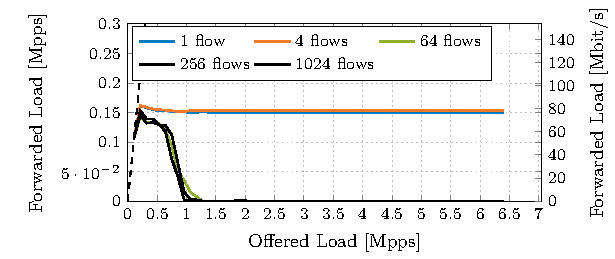
\includegraphics[width=0.5\linewidth]{figures/openvpn_fwd_setup1_60_bytes_variable_flows}
		\label{fig:openvpnfwdsetup160bytesvariableflows}
	}
	\subfloat[128 byte packets]{%
		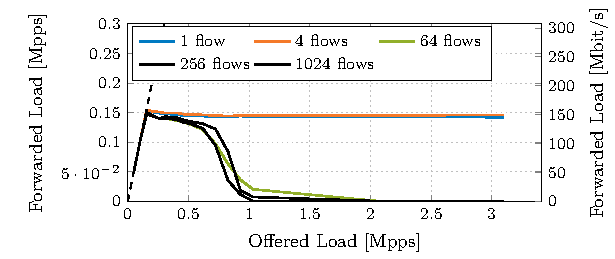
\includegraphics[width=0.5\linewidth]{figures/openvpn_fwd_setup1_124_bytes_variable_flows}
		\label{fig:openvpnfwdsetup124bytesvariableflows}
	}

	\subfloat[512 byte packets]{%
		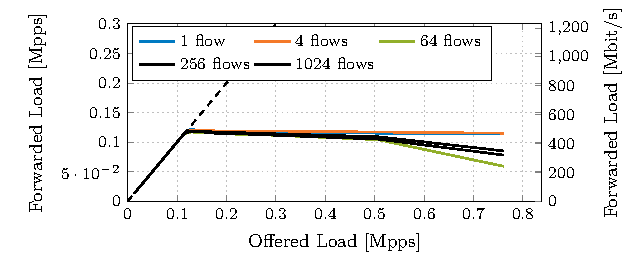
\includegraphics[width=0.5\linewidth]{figures/openvpn_fwd_setup1_508_bytes_variable_flows}
		\label{fig:openvpnfwdsetup508bytesvariableflows}
	}
	\subfloat[1510 byte packets]{%
		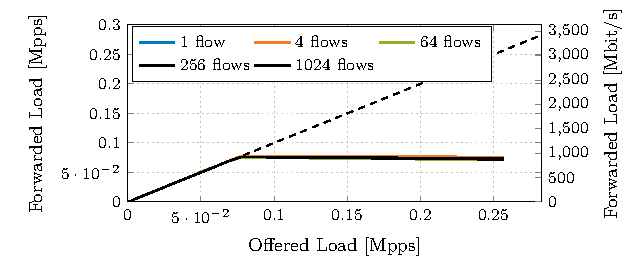
\includegraphics[width=0.5\linewidth]{figures/openvpn_fwd_setup1_1510_bytes_variable_flows}
		\label{fig:openvpnfwdsetup11510bytesvariableflows}
	}

	\caption{Forwarding performance of OpenVPN setup 1 with different packet sizes}
	\label{fig:openvpn-setup1-variablebytes-variableflows}
\end{figure}


\begin{figure}[h]
	\centering
	\subfloat[1 flow]{%
		\resizebox{0.33\columnwidth}{!}{%
			\begin{tabular}[htp]{|c|c|c|c|c|}%
\hline
\cellcolor{TUMBlue!0} CPU0 & \cellcolor{TUMBlue!93} CPU1 & \cellcolor{TUMBlue!0} CPU2 & \cellcolor{TUMBlue!0} CPU3 & \cellcolor{TUMBlue!0} CPU4 \\
\hline
\cellcolor{TUMBlue!0} CPU5 & \cellcolor{TUMBlue!0} CPU6 & \cellcolor{TUMBlue!0} CPU7 & \cellcolor{TUMBlue!0} CPU8 & \cellcolor{TUMBlue!0} CPU9 \\
\hline
\cellcolor{TUMBlue!0} CPU10 & \cellcolor{TUMBlue!0} CPU11 & \cellcolor{TUMBlue!0} CPU12 & \cellcolor{TUMBlue!0} CPU13 & \cellcolor{TUMBlue!0} CPU14 \\
\hline
\cellcolor{TUMBlue!0} CPU15 & \cellcolor{TUMBlue!0} CPU16 & \cellcolor{TUMBlue!0} CPU17 & \cellcolor{TUMBlue!0} CPU18 & \cellcolor{TUMBlue!0} CPU19 \\
\hline
\cellcolor{TUMBlue!0} CPU20 & \cellcolor{TUMBlue!0} CPU21 & \cellcolor{TUMBlue!2} CPU22 & \cellcolor{TUMBlue!0} CPU23 & \cellcolor{TUMBlue!0} CPU24 \\
\hline
\cellcolor{TUMBlue!0} CPU25 & \cellcolor{TUMBlue!0} CPU26 & \cellcolor{TUMBlue!0} CPU27 & \cellcolor{TUMBlue!0} CPU28 & \cellcolor{TUMBlue!0} CPU29 \\
\hline
\cellcolor{TUMBlue!0} CPU30 & \cellcolor{TUMBlue!0} CPU31 & \cellcolor{TUMBlue!93} CPU32 & \cellcolor{TUMBlue!0} CPU33 & \cellcolor{TUMBlue!0} CPU34 \\
\hline
\cellcolor{TUMBlue!0} CPU35 & \cellcolor{TUMBlue!0} CPU36 & \cellcolor{TUMBlue!0} CPU37 & \cellcolor{TUMBlue!0} CPU38 & \cellcolor{TUMBlue!0} CPU39 \\
\hline
			\end{tabular}
		}
	}
	%\hfill
	\subfloat[4 flows]{%
	\resizebox{0.33\columnwidth}{!}{%
		\begin{tabular}[htp]{|c|c|c|c|c|}%
			\hline
			\cellcolor{TUMBlue!1} CPU0 & \cellcolor{TUMBlue!93} CPU1 & \cellcolor{TUMBlue!0} CPU2 & \cellcolor{TUMBlue!0} CPU3 & \cellcolor{TUMBlue!0} CPU4 \\
			\hline
			\cellcolor{TUMBlue!0} CPU5 & \cellcolor{TUMBlue!0} CPU6 & \cellcolor{TUMBlue!0} CPU7 & \cellcolor{TUMBlue!0} CPU8 & \cellcolor{TUMBlue!0} CPU9 \\
			\hline
			\cellcolor{TUMBlue!0} CPU10 & \cellcolor{TUMBlue!0} CPU11 & \cellcolor{TUMBlue!0} CPU12 & \cellcolor{TUMBlue!0} CPU13 & \cellcolor{TUMBlue!93} CPU14 \\
			\hline
			\cellcolor{TUMBlue!0} CPU15 & \cellcolor{TUMBlue!0} CPU16 & \cellcolor{TUMBlue!0} CPU17 & \cellcolor{TUMBlue!0} CPU18 & \cellcolor{TUMBlue!0} CPU19 \\
			\hline
			\cellcolor{TUMBlue!0} CPU20 & \cellcolor{TUMBlue!0} CPU21 & \cellcolor{TUMBlue!0} CPU22 & \cellcolor{TUMBlue!0} CPU23 & \cellcolor{TUMBlue!0} CPU24 \\
			\hline
			\cellcolor{TUMBlue!0} CPU25 & \cellcolor{TUMBlue!93} CPU26 & \cellcolor{TUMBlue!0} CPU27 & \cellcolor{TUMBlue!0} CPU28 & \cellcolor{TUMBlue!0} CPU29 \\
			\hline
			\cellcolor{TUMBlue!0} CPU30 & \cellcolor{TUMBlue!0} CPU31 & \cellcolor{TUMBlue!93} CPU32 & \cellcolor{TUMBlue!0} CPU33 & \cellcolor{TUMBlue!0} CPU34 \\
			\hline
			\cellcolor{TUMBlue!0} CPU35 & \cellcolor{TUMBlue!93} CPU36 & \cellcolor{TUMBlue!0} CPU37 & \cellcolor{TUMBlue!0} CPU38 & \cellcolor{TUMBlue!0} CPU39 \\
			\hline
		\end{tabular}
		}
	}

	\subfloat[64 flows]{%
		\resizebox{0.33\columnwidth}{!}{%
			\begin{tabular}[htp]{|c|c|c|c|c|}%
	\hline
	\cellcolor{TUMBlue!93} CPU0 & \cellcolor{TUMBlue!93} CPU1 & \cellcolor{TUMBlue!93} CPU2 & \cellcolor{TUMBlue!93} CPU3 & \cellcolor{TUMBlue!93} CPU4 \\
	\hline
	\cellcolor{TUMBlue!0} CPU5 & \cellcolor{TUMBlue!93} CPU6 & \cellcolor{TUMBlue!93} CPU7 & \cellcolor{TUMBlue!93} CPU8 & \cellcolor{TUMBlue!0} CPU9 \\
	\hline
	\cellcolor{TUMBlue!0} CPU10 & \cellcolor{TUMBlue!93} CPU11 & \cellcolor{TUMBlue!0} CPU12 & \cellcolor{TUMBlue!0} CPU13 & \cellcolor{TUMBlue!93} CPU14 \\
	\hline
	\cellcolor{TUMBlue!93} CPU15 & \cellcolor{TUMBlue!93} CPU16 & \cellcolor{TUMBlue!93} CPU17 & \cellcolor{TUMBlue!93} CPU18 & \cellcolor{TUMBlue!93} CPU19 \\
	\hline
	\cellcolor{TUMBlue!93} CPU20 & \cellcolor{TUMBlue!93} CPU21 & \cellcolor{TUMBlue!93} CPU22 & \cellcolor{TUMBlue!0} CPU23 & \cellcolor{TUMBlue!0} CPU24 \\
	\hline
	\cellcolor{TUMBlue!93} CPU25 & \cellcolor{TUMBlue!93} CPU26 & \cellcolor{TUMBlue!93} CPU27 & \cellcolor{TUMBlue!93} CPU28 & \cellcolor{TUMBlue!93} CPU29 \\
	\hline
	\cellcolor{TUMBlue!93} CPU30 & \cellcolor{TUMBlue!93} CPU31 & \cellcolor{TUMBlue!93} CPU32 & \cellcolor{TUMBlue!93} CPU33 & \cellcolor{TUMBlue!93} CPU34 \\
	\hline
	\cellcolor{TUMBlue!0} CPU35 & \cellcolor{TUMBlue!93} CPU36 & \cellcolor{TUMBlue!93} CPU37 & \cellcolor{TUMBlue!93} CPU38 & \cellcolor{TUMBlue!93} CPU39 \\
	\hline
			\end{tabular}
		}
	}
	\subfloat[256 flows]{%
	\resizebox{0.33\columnwidth}{!}{%
		\begin{tabular}[htp]{|c|c|c|c|c|}%
\hline
\cellcolor{TUMBlue!93} CPU0 & \cellcolor{TUMBlue!93} CPU1 & \cellcolor{TUMBlue!93} CPU2 & \cellcolor{TUMBlue!93} CPU3 & \cellcolor{TUMBlue!93} CPU4 \\
\hline
\cellcolor{TUMBlue!93} CPU5 & \cellcolor{TUMBlue!93} CPU6 & \cellcolor{TUMBlue!93} CPU7 & \cellcolor{TUMBlue!93} CPU8 & \cellcolor{TUMBlue!34} CPU9 \\
\hline
\cellcolor{TUMBlue!93} CPU10 & \cellcolor{TUMBlue!93} CPU11 & \cellcolor{TUMBlue!93} CPU12 & \cellcolor{TUMBlue!93} CPU13 & \cellcolor{TUMBlue!93} CPU14 \\
\hline
\cellcolor{TUMBlue!93} CPU15 & \cellcolor{TUMBlue!93} CPU16 & \cellcolor{TUMBlue!93} CPU17 & \cellcolor{TUMBlue!93} CPU18 & \cellcolor{TUMBlue!93} CPU19 \\
\hline
\cellcolor{TUMBlue!64} CPU20 & \cellcolor{TUMBlue!93} CPU21 & \cellcolor{TUMBlue!93} CPU22 & \cellcolor{TUMBlue!93} CPU23 & \cellcolor{TUMBlue!93} CPU24 \\
\hline
\cellcolor{TUMBlue!93} CPU25 & \cellcolor{TUMBlue!93} CPU26 & \cellcolor{TUMBlue!93} CPU27 & \cellcolor{TUMBlue!93} CPU28 & \cellcolor{TUMBlue!93} CPU29 \\
\hline
\cellcolor{TUMBlue!93} CPU30 & \cellcolor{TUMBlue!93} CPU31 & \cellcolor{TUMBlue!93} CPU32 & \cellcolor{TUMBlue!93} CPU33 & \cellcolor{TUMBlue!93} CPU34 \\
\hline
\cellcolor{TUMBlue!64} CPU35 & \cellcolor{TUMBlue!93} CPU36 & \cellcolor{TUMBlue!64} CPU37 & \cellcolor{TUMBlue!64} CPU38 & \cellcolor{TUMBlue!93} CPU39 \\
\hline
		\end{tabular}
	}
}
\caption{CPU utilization of the DuT with setup 1 during 1000 Mbit/s load}
\label{fig:openvpn-setup1-60bytes-heatmap}
\end{figure}


\subsubsection{Cycle Analysis}
\label{sec:openvpn-cycle-analysis}

Next we analyze the efficiency of OpenVPN by calculating various relative metrics.

From our previous benchmarks we gather, that the impact of the number of flows is minimal for OpenVPN, as its processing rates are orders or magnitudes lower than what a Linux router can handle. To prevent negative interference from the IRQ handler we use single-flow traffic as the load, which is received on a single Rx queue on the DuT. 
To be able to make the most accurate attribution of CPU cycles, we also bind the OpenVPN process to a fixed core, so that is not accidentally scheduled on the same core the interrupts are handled.
For cycle measurements it is ideal if the applied load is just right, so that the DuT achieves its maximum processing rate, but is not yet overloaded. Since this rate is dependent on the packet size, we determined it for each setting.

\begin{figure}[h!]
	\centering
	\subfloat[Cycles per packet]{%
		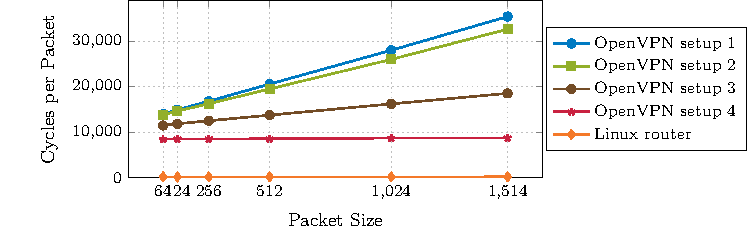
\includegraphics[width=0.9\linewidth]{figures/openvpn-cycles-per-packet}
		\label{fig:openvpn-cycles-per-packet}
	}
	
	\subfloat[Cycles per byte of packet]{%
		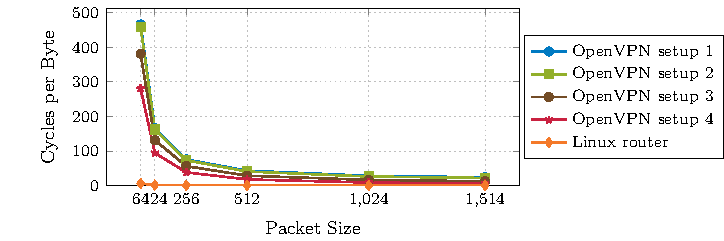
\includegraphics[width=0.9\linewidth]{figures/openvpn-cycles-per-byte}
		\label{fig:openvpn-cycles-per-byte}
	}

	\subfloat[Cycles per byte of payload]{%
		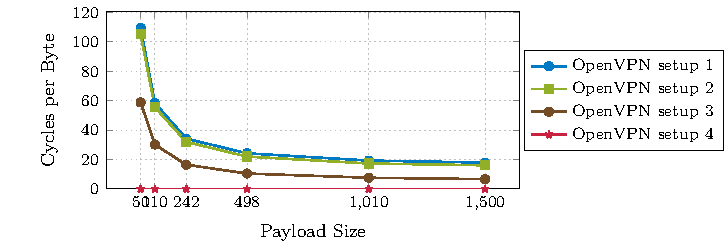
\includegraphics[width=0.9\linewidth]{figures/openvpn-cycles-per-byte-dynamic}
		\label{fig:openvpn-cycles-per-byte-dynamic}
	}
	
	\caption{Number of CPU cycles spend by OpenVPN under peak load}
	\label{fig:openvpn-cycle-analysis}
\end{figure}

Figure~\ref{fig:openvpn-cycle-analysis} (a) shows the cycles spend in total per packet processed. 
Firstly, it can be seen that the costs of OpenVPN absolutely dwarfs the overhead incurred by the underlying network stack, which is nearly constant at 140 - 170 cycles per packet. This again confirms our assessment, that the bottleneck of OpenVPN does not lie within the Linux network or driver stack.
Choosing the AES-256 cipher (setup 1) with a larger block size compared to AES-128 (setup 2), incurs a measurable overhead of 1.5\% to 8\%. The overhead is smallest for 64 byte packets (+212 cycles) and increases with packet size (+2780 cycles for 1514 byte).
A much bigger impact has the data integrity mechanism. Disabling HMAC-SHA256 signatures reduces the costs by $\sim$40\%. This rather large value can be explained by the way OpenVPN calculates the signature: it is essentially a second, separate pass over the encrypted payload and not generated on-the-fly~\cite{openvpn-encrypt-v1}.

Setup 4 has the most distinct curve, as the costs per packet do not increase with larger packet sizes, but remain constant. This can be attributed to the configuration of the setup, which does neither encrypt data, nor does it generate signatures. With this work minimizing setting, the static overhead of handling a packet in OpenVPN has been found at 8500 cycles per packet. Unless this overhead cannot be reduced, the maximum processing rate lies at $\frac{2.2\ \textrm{GHz}}{8500\ \textrm{cycles}} = 0.26\ \textrm{Mpps}$ on the tested hardware. In Paragraph~\ref{sec:openvpn-userspace} we further analyze this overhead. 

Figures~\ref{fig:openvpn-cycle-analysis} (b) and (c) give more insight on the dynamic processing costs. In (b) the required cycles per byte of packet data, depending on the total packet length, are displayed. The sharp decrease at 128 and 256 bytes explains, why OpenVPN is only able to achieve high throughput at large packet sizes.
Figure (c) refines this metric by subtracting the static per-packet overhead and by ignoring the Ethernet header fields in the payload calculation. In a L3 VPN they do not get encrypted. The resulting values represent the costs of the cryptographic operations per by byte of data. It can be seen, that these are still comparatively huge for small data chunks at 60 to 100 cycles/byte, but amortize with larger buffers to under 20 cycles/byte. Compared to other benchmarks and implementations this is a low value~\cite{bench.cr.yp.to}, but confirms that the encryption is not the main bottleneck of OpenVPN, at least not a larger packet sizes.

%\begin{equation}
%\textrm{text} * 5
%\frac{num}{den}
%\end{equation}


\subsubsection{Drawbacks of Running in User-space}
\label{sec:openvpn-userspace}

OpenVPN enjoys higher portability across operation systems by completely running in user-space, as opposed to direct Kernel integration like IPsec.
%There are some drawbacks of running in user-space. In the stack traces some functions can be found, that do not occur in other VPNs. 
There are however, some drawbacks that come with this architectural decision.

\begin{table}
	\centering
	\resizebox{0.5\linewidth}{!}{
		\begin{tabular}{rl}
			\toprule
			Percentage & Symbol \\
			\midrule
			%		 6.49\%&[kernel.kallsyms] &[k] entry\_SYSCALL\_64 \\
			%		5.73\%&[kernel.kallsyms] &[k] entry\_SYSCALL\_64\_fastpath \\
			%		4.62\%&[kernel.kallsyms] &[k] \_raw\_spin\_lock\_irqsave \\
			%		3.25\%&[kernel.kallsyms] &[k] \_raw\_spin\_lock\\
			%		3.17\%&[kernel.kallsyms] &[k] tun\_do\_read\\
			%		2.54\%&[kernel.kallsyms] &[k] tun\_chr\_poll\\
			%		2.26\%&[kernel.kallsyms] &[k] do\_sys\_poll\\
			%		2.22\%&[kernel.kallsyms] &[k] copy\_user\_generic\_unrolled\\
			%		2.08\%&libcrypto.so.1.0.0&[.] 0x000000000009f8cd\\
			%		1.82\%&libcrypto.so.1.0.0&[.] SHA1\_Final\\
			%		1.66\%&[kernel.kallsyms] &[k] \_\_fget\_light\\
			%		1.65\%&libcrypto.so.1.0.0&[.] SHA1\_Update\\
			%		1.50\%&[kernel.kallsyms] &[k] \_\_skb\_recv\_datagram\\
			%		1.50\%&[kernel.kallsyms] &[k] entry\_SYSCALL\_64\_after\_swapgs\\
			%		1.42\%&[kernel.kallsyms] &[k] fib\_table\_lookup\\
			%		1.32\% & [kernel.kallsyms] &[k] \_\_free\_page\_frag\\
			%		1.11\%&[kernel.kallsyms] &[k] copy\_user\_enhanced\_fast\_string\\
			%		1.01\%&[kernel.kallsyms] &[k] \_\_lock\_text\_start\\
			11.60\% & [k] entry\_SYSCALL\_64\_fastpath \\
			10.37\% & [k] entry\_SYSCALL\_64\\
			4.65\% & [k] \_raw\_spin\_lock\\
			3.95\% & [k] do\_sys\_poll \\
			3.37\% & [k] \_raw\_spin\_lock\_irqsave\\
			2.90\% & [k] copy\_user\_generic\_unrolled\\
			2.31\% & [k] tun\_chr\_poll\\
			2.26\% & [k] fib\_table\_lookup\\
			2.05\% & [k] \_\_lock\_text\_start \\
			1.89\% & [k] \_\_fget\_light\\
			\bottomrule
		\end{tabular}
	}
	\caption{Top 10 most run functions in OpenVPN setup 4}
	\label{tab:openvpn-stacktrace}
\end{table}

\subitem{\textbf{Switching from User-mode to Kernel-mode}}

OpenVPN receives and sends its data via the UNIX socket API, as it has no low-level access to drivers from user-space. The API is implemented as system calls (syscalls), where the privilege level is temporarily bumped to kernel-mode and Kernel functions are run. Upon entry of such a syscall, the validity of the parameters have to be checked and the CPU registers of the calling process are saved.
This separation is important for security, but incurs an overhead if system functions are frequently used. 
In Table~\ref{tab:openvpn-stacktrace} we can see, that in fact 13\% of the processing time is spend in the entry functions \texttt{entry\_SYSCALL\_64\_fastpath} and \texttt{entry\_SYSCALL\_64}. Following the call chain, we found that these come from calls to \texttt{read()}, \texttt{sendto()} and \texttt{poll()}.

\subitem{\textbf{TODO title: Address space Separation}}

Another overhead comes from the way sockets are implemented on Linux. 
Upon a \texttt{send()} syscall the data is not immediately given to a NIC and send out on the wire. To gain optimizations from batching and reduce interrupt rates, the data is first gathered in the sockets send buffer and processed by the Kernel later at an opportune moment. Figure~\ref{fig:socket-send-buffers} vizualizes this concept.

\begin{figure}[h]
	\centering
	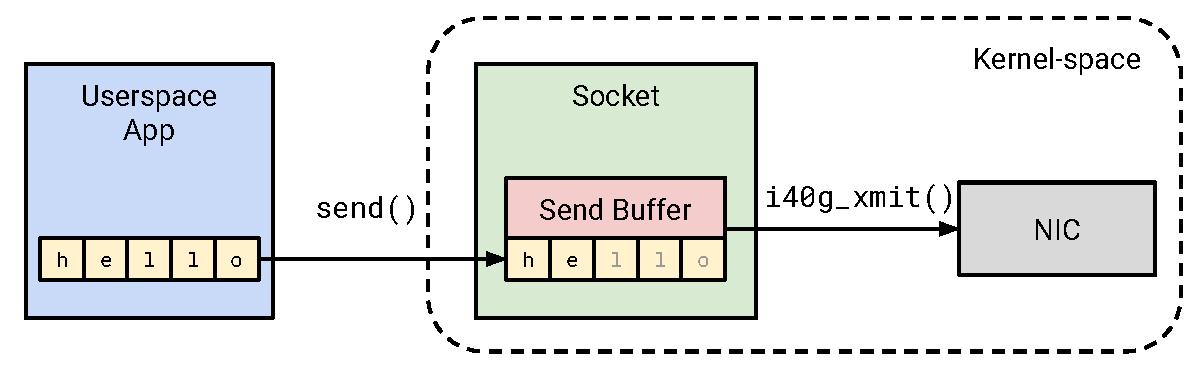
\includegraphics[width=0.7\linewidth]{figures/socket-send-buffers}
	\caption{Socket send buffers on Linux}
	\label{fig:socket-send-buffers}
\end{figure}

Since the API specifies that a user-supplied buffer can be reused after a successful \texttt{send()} call, the data actually has to be copied into the socket's buffer. The converse is true for received data, which is copied from driver memory into the user address space.
The costs of this memory copying manifests in the entry \texttt{copy\_user\_generic\_unrolled} of the performance measurement shown in Table~\ref{tab:openvpn-stacktrace}, where 2.9\% of the cycles are spend.


[stackplot detailed cpu usage]

\begin{figure}[h]
	\centering
	\subfloat[1 Flow]{%
		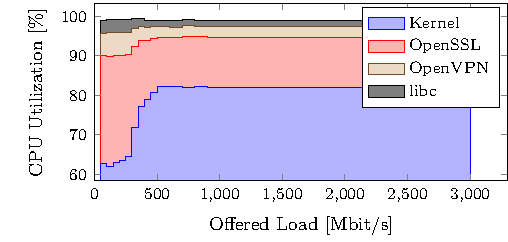
\includegraphics[width=0.5\linewidth]{figures/openvpn_fwd_setup1_60_bytes_1_flows_all_cpu}
		\label{fig:openvpnfwdsetup160bytes1flowsallcpu}
	}
	\subfloat[4 Flows]{%
		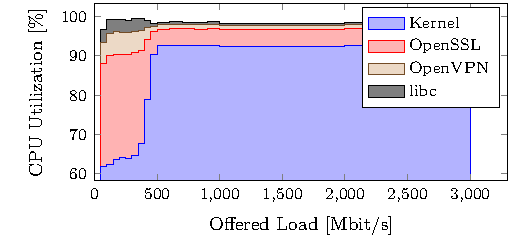
\includegraphics[width=0.5\linewidth]{figures/openvpn_fwd_setup1_60_bytes_4_flows_all_cpu}
		\label{fig:openvpnfwdsetup160bytes4flowsallcpu}
	}

	\subfloat[64 Flows]{%
		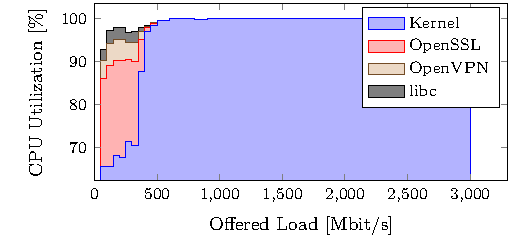
\includegraphics[width=0.5\linewidth]{figures/openvpn_fwd_setup1_60_bytes_64_flows_all_cpu}
		\label{fig:openvpnfwdsetup160bytes64flowsallcpu}
	}
	\subfloat[1024 Flows]{%
		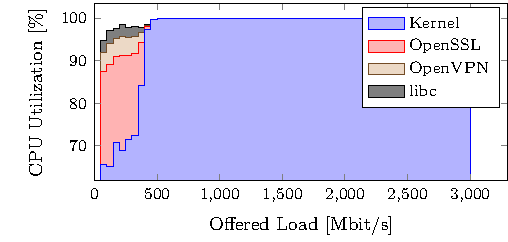
\includegraphics[width=0.5\linewidth]{figures/openvpn_fwd_setup1_60_bytes_1024_flows_all_cpu}
		\label{fig:openvpnfwdsetup160bytes1024flowsallcpu}
	}
	\caption{CPU utilization of DuT running OpenVPN setup 1 with 60 bytes packets and varying flows}
	\label{fig:openvpn-setup1-64-byte-cpu-util}
\end{figure}

\begin{figure}[h]
	\centering
	\subfloat[1 Flow]{%
		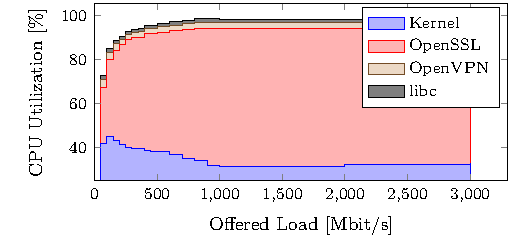
\includegraphics[width=0.5\linewidth]{figures/openvpn_fwd_setup1_1510_bytes_1_flows_all_cpu}
		\label{fig:openvpnfwdsetup11510bytes1flowsallcpu}
	}
	\subfloat[4 Flows]{%
		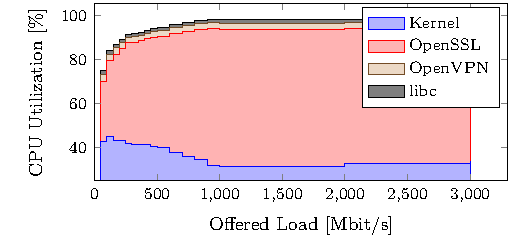
\includegraphics[width=0.5\linewidth]{figures/openvpn_fwd_setup1_1510_bytes_4_flows_all_cpu}
		\label{fig:openvpnfwdsetup11510bytes4flowsallcpu}
	}
	
	\subfloat[64 Flows]{%
		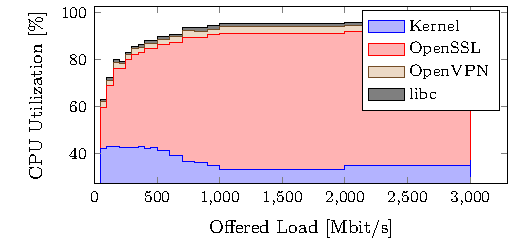
\includegraphics[width=0.5\linewidth]{figures/openvpn_fwd_setup1_1510_bytes_64_flows_all_cpu}
		\label{fig:openvpnfwdsetup11510bytes64flowsallcpu}
	}
	\subfloat[1024 Flows]{%
		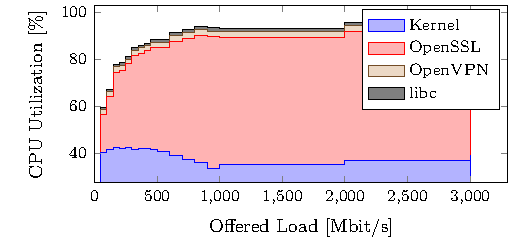
\includegraphics[width=0.5\linewidth]{figures/openvpn_fwd_setup1_1510_bytes_1024_flows_all_cpu}
		\label{fig:openvpnfwdsetup11510bytes1024flowsallcpu}
	}
	\caption{CPU utilization of DuT running OpenVPN setup 1 with 1514 bytes packets and varying flows}
	\label{fig:openvpn-setup1-1510-byte-cpu-util}
\end{figure}

[graph: openvpn setup 1, 1514 bytes, ]

\subsection{OpenSSL Benchmark}
OpenVPN does not supply its own cryptographic primitives, but relies on the high-level OpenSSL API named EVP (EnVeloPe) for all cryptographic operations.
In Section~\ref{sec:openvpn-cycle-analysis} we show that encryption takes a non-negligible amount of time per packet.

\begin{figure}[h!]
	\centering
	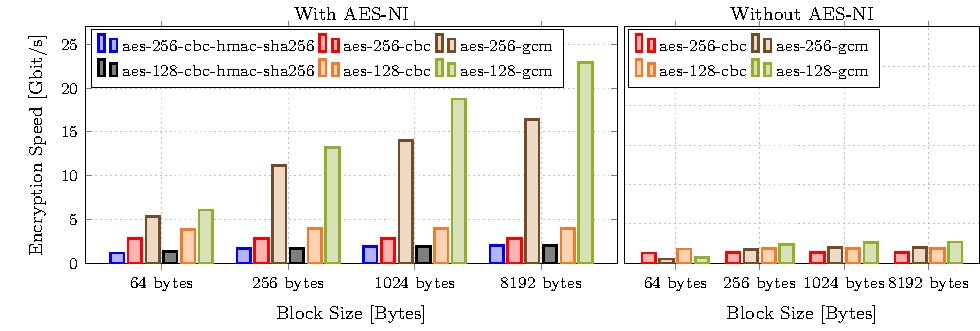
\includegraphics[width=1.0\linewidth]{figures/openssl_ciphers}
	\caption{OpenSSL encryption speeds for AES ciphers depending on AES-NI support}
	\label{fig:opensslciphers}
\end{figure}

Nonetheless, there is some benefit in having a detailed look at the underlying primitives. Firstly, OpenVPN does not support every cipher implemented by OpenSSL. In particular the AES GCM variants are not exposed in static key mode. By benchmarking them too, we gain a broader view and can make a prediction about potential improvements. Another reason is, that neither OpenVPN, nor OpenSSL provide a switch to en- or disable the AES-NI accelerated functions, or even a simple indication if they are used. Other research shows that the availability of this instruction set extension is crucial for good performance~\cite{raumer2016efficient}\cite{lackovic2017performance}. In this benchmark we can explicitly control this and observe the effects.

Listing~\ref{lst:openvpn-openssl-benchmark} shows how to modify the OpenSSL processor capabilities vector~\cite{openssl-manpage-proc-cap-vector} by negating the 57th bit, so that only the non-AES-NI supporting implementations are selected.

\begin{lstlisting}[caption={Snippet to benchmark OpenSSL with AES-NI disabled},captionpos=b,label={lst:openvpn-openssl-benchmark},language=bash]
OPENSSL_ia32cap="~0x200000000000000" openssl speed -evp <cipher>
\end{lstlisting}

In Figure~\ref{fig:opensslciphers} the results are displayed for a selection of ciphers and how they perform on different block sizes. The left side shows the encryptions speeds with AES-NI enabled, on the right side it is disabled.
Several conclusion can be drawn from this benchmark. 
The 128-bit block size ciphers are always equal to or faster than its 256-bit versions, but except for AES-GCM, the difference is within 10\%, which matches the results in Section~\ref{sec:openvpn-cycle-analysis}.
Fastest by a wide margin are the newer GCM variants, which are not available in OpenVPN static key mode. They outperform CBC modes by a factor of 1.5 to 10. We can confirm that AES-NI is  indeed very important to performance. No cipher implementation even reaches 2.5 Gbit/s without this instruction set extension.


\subsection{Optimizations}
\subsubsection{recv/snd buffer sizes, TUN queue length}
--sndbuf, --rcvbuf, --txqueuelen, --fast-io, --tun-mtu

[Graph: sendbuffer vs fwd rate, no enc or auth, ]


%TODO: combine in initial results
%\subsubsection{taskset \& rx queues}
%The Linux Kernel softirq processes performing work in response to interrupts.
%As they are interacting with the hardware, they are prioritized higher than user-space processes by the scheduler. Under heavy load these can monopolize the CPU completely, so that no other process gets a chance to run. An example for this behavior can be seen in Subfigures~\ref{fig:openvpn-setup1-64-byte-cpu-util} (c) and (d), where the Rx handler of the NIC driver increasingly blocks out the VPN process. This results in a reduced or even zero processing rate as displayed in Figure~\ref{fig:openvpn-setup1-variablebytes-variableflows}.
%As a possible solution one can deviate from the default 1:1 mapping of queues to cores and leave on core free by reducing the number of queues.
%With a tool like \texttt{taskset}, the OpenVPN process can the be explicitly bound to this free CPU. 
%Figure~\ref{} shows the measured processing rates for 64 byte packets in 256 flows and compares it with the standard queue setup. It can be seen that the peak performance does not change when the process is bound to the free core. Only once the DuT is overloaded the improvement becomes visible. Where the  throughput previously drastically decreased once more than 0.75 Mpps arrived, it now remains at XXX.
%
%This shows that an alternative queue configuration can help to elevate the throughput loss under high load.


%\subsection{Frequency Scaling}
%Modern CPUs have a wide array of power states and frequencies that they can run on. The Intel Xeon E... has a nominal frequency of 2.2 GHz, but can increase the clock rate for select cores to up to 3.1 GHz through a mechanism called TurboBoost.
%Single-threaded applications often benefit more from a higher clock rate, than from an abundance of cores. 
%For this benchmark we again bound the OpenVPN process to a specific core and fixed it frequency to increasing values. In Figure\ref{} it can be seen, that OpenVPN does indeed perform better at higher rates. , although 


\subsection{Multiple Instances}
The single-threaded design of OpenVPN limits its performance to very low levels compared to IPsec and WireGuard, as some VPN tasks, e.g. encryption, simply need raw CPU processing power to scale.

While multi-threading has been on the development roadmap of the official OpenVPN application since 2010, very little has change since then. According to the developers, this is partly to blame on the current event-system implementation, which is only partly asynchronous and requires that, e.g. resource freeing, happens synchronously\cite{}.
They estimate that introducing multi-threading requires a complete rewrite of the I/O system and have postponed this to OpenVPN 3.0.
For now this leaves users with multi-processing as a scaling vector. This is not a build-in feature of OpenVPN, but has to be setup manually with external tools. 
The approach is conceptually similar to the multi-SA technique for IPsec presented in Section~\ref{}: The incoming traffic is split up according to its destination address via multiple routes and processed by different processes.
In this case, we spawn multiple OpenVPN instances, each handling a distinct /32 subnet. Contrary to IPsec, some additional steps and workarounds for limitations in OpenVPN are required, as shown in Listing~\ref{lst:openvpn-multiprocess-script}.

\begin{lstlisting}[caption={Script to set up multi-process OpenVPN},captionpos=b,label={lst:openvpn-multiprocess-script},language=bash]
ethtool -L ens3f0 combined 4
IP_LOW=2; CPU_LOW=4;
for i in $(seq 0 1 $COUNT)
do
	ip a add 10.1.0.$(expr $IP_LOW + $i)/24 dev ens4f0
	taskset -c $(expr $CPU_LOW + $i) openvpn --verb 3 \
		--dev tun$i --proto udp --cipher AES-256-CBC --auth SHA256 \
		--local 10.1.0.$(expr $IP_LOW + $i) --remote 10.1.0.254
		--route 10.2.0.$(expr 2 + $i) 255.255.255.255 
		--ifconfig 192.168.0.1 192.168.0.$(expr 2 + $i)
		--secret ~/static.key &
done
\end{lstlisting}
Firstly, we reduce the number of NIC queues to 4 and bind them to the first four cores, so that the interrupt handlers do not interfere with the OpenVPN processes.
In Line 5 additional IP addresses on the outgoing interface have to be configured for each instance. Otherwise they would fail with an \texttt{EADDRINUSE} (address already in use by other socket) error.
With \texttt{taskset} we prevent unnecessary CPU migrations and contention for processing power by cleanly separating them of the kernel threads. Having each process bound to a different CPU core limits energy efficiency as these cores can not be put in low power states during low load, but this may not be a concern in high throughput setups.

\begin{figure}[h]
	\centering
	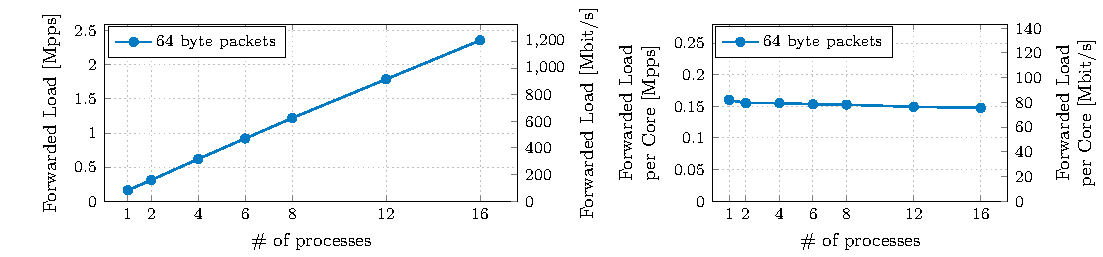
\includegraphics[width=1\linewidth]{figures/openvpn_multi_process_60_bytes_variable_flows}
	\caption{Processing rates with multiple OpenVPN instances}
	\label{fig:openvpnmultiprocess60bytesvariableflows}
\end{figure}

Figure~\ref{fig:openvpnmultiprocess60bytesvariableflows} (a) shows the improvements in processing rate that can be made, depending on the numbers of processes spawned. The number of flows in the offered traffic exactly matches the number of processes, to get an even work distribution.
Since each worker process is essentially independent with its own TUN device, route and IP address, we see the expected near linear speedup. For traffic of 64 byte packets the rates increase from the already known 0.16 Mpps in single-instance mode, to 2.36 Mpps with 16 processes. The throughput consequently also grows to 1.2 Gbit/s. This means the DuT is able to handle an entire Gigabit link of incoming traffic.
To score the effectiveness of additional resources and to forecast the scaling capabilities beyond 16 processes, the processing rates per core are displayed in Figure~\ref{fig:openvpnmultiprocess60bytesvariableflows} (b). While there is a measurable reduction, especially in the step from one to two processes, the rate only decreases marginally after that and stays close to 0.148 Mpps per added process.
Provided one additional free CPU cores, it would be possible to scale this up further.

\subsubsection{Caveats}
While some performance gains can be made, this approach is not without serious drawbacks.
Firstly, the incoming traffic must be evenly distributed on the configured routes, since a single instance is not faster than before and can still be the bottleneck. In real-world networks this often not the case as a few "elephant" flows dominate bandwidth-wise.
Since the filter mechanism is basically the Linux routing table, the granularity of a filter is quite low. /32 subnets (a single destination IP) is the finest setting. 
Consequently this means, that the uplink capacity to a single host is still limited to 0.16 Mpps. In an environment where many hosts push data to a single server, this approach could be much less applicable.
%- configuration overhead
There also is an additional configuration \& maintenance burden to be taken. Each instance needs a free IP address and has to be started, monitored and stopped.
%- static, can't react to surges
Lastly, this setup is completely static and does not react sudden traffic changes in form or amount. A smarter implementations could monitor the processed traffic and continuously update the filter routes or scale the number of processes.

\section{WireGuard}

	\subsection{GSoC Performance Improvements}
	
	Google Summer of Code is an annual program to bring students to open-source software development under a mentorship. During 2018 the three students Jonathan Neuschäfer, Thomas Gschwantner and Gauvain  Roussel-Tarbouriech participated in the program and worked on WireGuard with the goal to improve performance and do measurements. %TODO: cite
	
	They created a number of commits, of which X got merged. Due to time constraints and other problems they could not perform extensive profiling and performance measurement. Consequently they did not include detailed documentation in their report about the performance improvements they could achieve.
	
	The next section lists their performance-related changes, explains their high-level goals, benchmarks them against the developed criteria and analyzes the improvements. In the case of unchanged or even decreased performance, I explain why the approach does not work.
	
	Since the changes have been made independently and at different times, they do not always base upon the same code version and include commits of other developers, which could influence performance. To evaluate the changes fairly, not the absolute differences between them will be compared. Instead, each change will be evaluated against the latest version directly before the change. The relative improvements can then be compared against each other fairly.
	
	\begin{table}[h]
		\centering
		\begin{tabular}{l c c}
			Tree & Reference & Improved \\ 
			\hline 
			\texttt{tg/mpmc\_ring} &  &  \\ 
			\texttt{jn/mpmc-wip} & dfd9827 &  5e4689d\\ 
			\texttt{tg/mpmc-benchmark} & dfd9827  & 6f909b2 \\ 
			Prefix-Trie & & \\
			NAPI & & \\
			Hashtable & & \\
		\end{tabular}
		\caption{Commit hashes}
		\label{tab:gsoc-commits}
	\end{table}
	
	Table~\ref{tab:gsoc-commits} shows the exact hashes of the tested commits and the baseline they are compared against.
	
	\subsubsection{MPMC Queue}
	[They] replaced the spin-lock based ring buffer WireGuard uses to distribute packets to workers. They choose a lock-free multi-producer multi-consumer (MPMC) implementation based on the ConcurrencyKit \cite{todo}. 
	
	As the students could not finish the implementation in time, it has not been merged into the master branch. There exist three branches which contain MPMC implementations: \texttt{tg/mpmc\_ring} is the initial version of Thomas Gschwantner, \texttt{jn/mpmc-wip} contains the combined efforts of him and Jonathan Neuschäfer and \texttt{tg/mpmc-benchmark} extends the previous version by a simple benchmark script and patch to fix scheduling of producers by disabling preemption during enqueue operations. A fix that apparently was needed because of deadlocks.
	
	It should be noted that both \texttt{jn/mpmc-wip} and \texttt{tg/mpmc-benchmark} did not compile cleanly due to errors.
	The first is an erroneous include of a file which does not exist. After consulting the Linux Kernel documentation I concluded that this statement is most likely just a minor mistake and removed it, upon which the code compiled without errors or warnings.
	The second error uses a function which has been deprecated since Kernel version 3.14~\cite{bibid}. Since the test systems are on Kernel version 4.XX, I unconditionally replaced the call with its replacement function.
	Listing~\ref{lst:include-fix} shows the exact changes made.
	
	\begin{lstlisting}[caption={Patches to compile MPMC commits},captionpos=b,label={lst:include-fix}]
diff --git a/src/mpmc_ptr_ring.h b/src/mpmc_ptr_ring.h
index da9393e..e035b9e 100644
--- a/src/mpmc_ptr_ring.h
+++ b/src/mpmc_ptr_ring.h
@@ -44,7 +44,7 @@
#include <linux/compiler.h>
#include <linux/errno.h>
#include <linux/log2.h>
-#include <linux/processor.h>
+// #include <linux/processor.h>
#include <linux/slab.h>
#include <linux/stddef.h>

diff --git a/src/mpmc_ptr_ring.h b/src/mpmc_ptr_ring.h
index a4f8344..2cee50a 100644
--- a/src/mpmc_ptr_ring.h
+++ b/src/mpmc_ptr_ring.h
@@ -47,7 +47,9 @@
//#include <linux/processor.h>
#include <linux/slab.h>
#include <linux/stddef.h>
+#include <linux/preempt.h>

+#define preempt_enable_no_resched() preempt_enable()

struct mpmc_ptr_ring {
/* Read-mostly data */
	\end{lstlisting}
	
	\begin{figure}
		\centering
		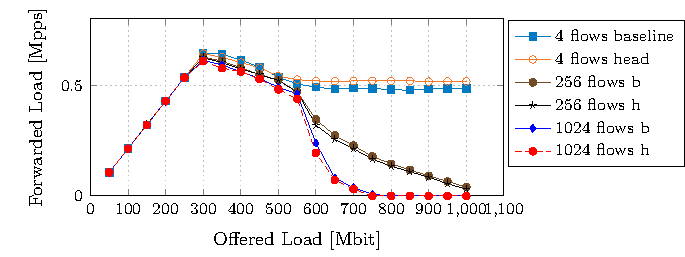
\includegraphics[width=1\linewidth]{figures/mpmc-wip-wg0-compare-encrypt-64bytes-omastar}
		\caption{Comparison of processing rates for \texttt{mpmc-wip} branch on WireGuard device}
		\label{fig:mpmc-wip-wg0-compare-encrypt-64bytes-omastar}
	\end{figure}
	
	Figure~\ref{fig:mpmc-wip-wg0-compare-encrypt-64bytes-omastar} show the improvements 
	
	\subsubsection{Endianness in Prefix-Trie}
	
	\subsubsection{NAPI}
	
	\subsubsection{GRO}
	
	\subsubsection{Peer Hashtable}
	
\section{MoonWire}
TODO

\chapter{Performance Model for VPN Implementations}
\label{chap:perf_model}
This Chapter presents the developed performance model for VPN implementations. 

Implementations are wildly different, but share some common functionality as part of their VPN operation. The following sections dissect and extract the core tasks of a VPN. For these core task I then define bounds that can be used to estimate performance numbers. These bounds are based on experimentation, benchmarks results and calculations.

\section{Major Tasks}
All VPNs are comprised of a number of task they complete to provide their functionality.

\subsection{Network Driver \& Stack}
Before a packet reaches the VPN code, buffers have to be allocated, data has to be received and fields have to be validated. The same goes for the send path, where the packet passes through multiple layers until it is delivered over the wire.

While a VPN implementation usually has no influence over the decision which network stack is used, a major chunk of the systems performance is decided at this low level.
If the NIC driver is slow or inefficient, then the upper application can do very little to nothing to redeem this and still be fast.

The severity of this can be illustrated by the following example calculation. For a given line rate of packets per second that have to be processed and a given CPU model and clock rate, concrete time budgets can be calculated for each packet. Table~\ref{tab:todo} shows such budgets for X Mpps and a modern Intel Xeon XXX cpu. It lists the average timings of network driver operations and data accesses to cache and memory. 

[cycle budget per packet table]

It can be seen that these costs are not to be neglected and can easily determine the systems overall performance.

Since a packet has to be passed twice, receive and send path, through this stack, we can establish the following equation for this part of the performance model: 

\begin{equation}\label{eq:cost}
asd
\end{equation}

Figure X shows the correlation of processing time spend on rx/tx and the systems maximum forwarding rate.

\begin{figure}[h]
	\centering
	\begin{tikzpicture}
		\begin{axis}[
			scale only axis,
			height=4cm,
			width=7cm,
			]
			\addplot[mark=none]{x^2};
		\end{axis}
	\end{tikzpicture}
	\caption{heading}
\end{figure}


It is obvious that a VPN will not deliver packets faster than the underlying network stack allows. 
Although optimizations like GRO can elevate the pressure to some degree.

\subsection{Memory Management}
\subsection{Cryptographic Operations}
\subsection{Multicore Synchronization}
\subsection{Data Structures}


\section{Influencing Factors}
	\subsection{Network Stack \& Drivers}
	\subsection{Memory Management}
	\subsection{Multi-core Scaling}
	\subsection{Cryptographic Ciphers}
	\subsection{Data Structures}
		Queues
		Routing
		State Storage \& Lookup


\chapter{Conclusion}
\label{chap:conclusion}
\section{Future Work}
	Implement better queuing: CODel

\appendix
\chapter{Supplementals}

\listoffigures
\listoftables

\chapter{Appendix}

foo


\printacronyms[heading=chapter,name=List of Acronyms]
\clearpage
\pagestyle{thesischapter}

\cleardoublepage
%\printbibliography[heading=bibintoc]
\printbibliography

%\cleardoublepage
\clearpage
\pagestyle{empty}
%\mbox{}
%\clearpage

\end{document}


